\documentclass[a4paper,10pt]{report}
%[12pt,svgnames]{beamer}
%********************************************************
%**************** Chargement des paquets ****************
%********************************************************
%-------------------------------------%******************
%-------------------------------------%   MISE EN PAGE  *
%-------------------------------------%******************
\usepackage[a4paper, left=2.5cm, width=16cm, height=25.4cm, includehead, includefoot, headheight=13.6pt]{geometry}
\usepackage{multicol}                 % Ecrire en colones \begin{multicols}{2} \end{multicols}
\usepackage[explicit, clearempty]{titlesec}	  	  % Titres personalisables
\usepackage{titletoc}                 % Table des matières
\usepackage[hidelinks]{hyperref}      % Lien vers les chapitres en table de matières
\hypersetup{pdfencoding=unicode}
\usepackage{fancyhdr}		          % En-tête et pied de page
\usepackage{enumitem}                 % Enumérations
\usepackage{fancyvrb}                 % augmente les possibilités de verbatim
\usepackage{answers}                  % Solutions des exerices en fin de chapitre
\usepackage[dvipsnames]{xcolor}
%\usepackage[cache=false]{minted}
\usepackage{tcolorbox}
\tcbuselibrary{minted,skins,theorems}
\tcbset{listing engine=minted}
%\usepackage{nameref}
%-------------------------------------%******************
%-------------------------------------%    CARACTERES   * 
%-------------------------------------%******************
\usepackage{fontspec}   
  \setmonofont[Scale=MatchLowercase,BoldFont={Inconsolatazi4 Bold}]{Inconsolatazi4}
  \newfontfamily\inconsola{Inconsolatazi4}
  \newfontfamily\greekfont[Script=Greek, Scale=MatchUppercase, Ligatures=TeX]{Arial}
  \newfontfamily\cursive[Ligatures=TeX]{dancing-script-ot.ttf}
  \newcommand{\textgreek}[1]{\bgroup\greekfont#1\egroup}
\usepackage{polyglossia}
  \setmainlanguage{french}
  \setotherlanguage{english}
%-------------------------------------%******************
%-------------------------------------%  MATHEMATIQUES  *
%-------------------------------------%******************
\usepackage{amsmath,                  % Mise en forme de formules, équations
            amsfonts,                 % Symboles, tailles adaptées, Fraktur, Cyrillic
            amssymb,                  % Symboles mathématiques (e.g. \mathbb{R} )
            amsthm}                   % Personalisation des théorèmes
\usepackage{mathrsfs}                 % Pour l'écriture cursive \mathscr{C}
\usepackage[np]{numprint}	          % Pour l'écriture des nombres \np{3250.58}
%-------------------------------------%******************
%-------------------------------------%     TABLEAUX    *
%-------------------------------------%******************
\usepackage{array,                    % Tableaux plus riches que tabular simple
            multirow,                 % Pour fusionner des lignes
            makecell}	              % Autres macro de manipulation des lignes
\usepackage{colortbl}	              % Couleurs de fond
%-------------------------------------%******************
%-------------------------------------%    GRAPHIQUES   *
%-------------------------------------%******************
\usepackage{color}
%-------------- TIKZ -----------------
\usepackage{pgf,tikz}			 	  % Dessinner avec tikz
\usetikzlibrary{shapes,               % d'autres formes
           decorations.pathreplacing, % pour les accolades
           calc,                      % Calculs de coordonnées entre $ $
           patterns,                  % Pour les remplissages
           intersections,             % Calcul d'intersections de chemins
           automata,
           positioning,
           graphs,
           matrix,
           shadows.blur,
           shadings,
           shapes.callouts,
           shapes.arrows,
           angles,
           arrows,
           decorations.text,
           shapes.gates.logic.US,
           shapes.gates.logic.IEC}
\pgfdeclarelayer{background}
\pgfsetlayers{background,main}
\usepackage[tikz]{bclogo}             % Les boites avec logo ( dans \Cours )
\usepackage{graphicx}	              % Inclusion d'images
\usepackage[oldvoltagedirection]{circuitikz} % Pour les portes logiques

\let\emph\relax
\DeclareTextFontCommand{\emph}{\bfseries\color{Blue}}

\definecolor{jaune}{RGB}{255,255,0}
\definecolor{bleu}{RGB}{0,112,192}
\definecolor{html}{RGB}{221,78,37}
\definecolor{css}{RGB}{12,111,178}
\definecolor{js}{RGB}{221,157,39}
\definecolor{SQL}{RGB}{0,0,0}
%********************************************************
%************ PERSONALISATIONS ET RACOURCIS *************
%********************************************************
\usepackage{xifthen}                  % pour les tests \isempty des commandes
\pagestyle{fancy}
\fancypagestyle{plain}{\fancyfoot[C,L,R]{}\renewcommand{\headrulewidth}{0pt}\fancyhead[C,L,R]{}}
\fancypagestyle{plain}{\fancyfoot[R]{\thepage}\renewcommand{\headrulewidth}{0pt}\fancyhead[C,L,R]{}}
\fancyhead{}\lhead{\leftmark}\renewcommand{\headrulewidth}{0.1pt}\rhead{\thepage}
\lfoot[]{}\cfoot{}\rfoot[]{}
\newcommand\rubrique{rubrique}
\renewcommand{\chaptermark}[1]{\markboth{\rubrique > #1}{}}
\titleformat{name=\chapter, numberless}[display]
    {\LARGE\bfseries\filright}
    {\begin{tikzpicture}
    \node[draw,text width = \textwidth-\pgflinewidth-10pt,inner sep = 5pt,align = center](Ch){\strut\begin{minipage}{0.66\textwidth}\centering#1\end{minipage}};
    \end{tikzpicture}}
    {0pt}
    {}[\small]
\titleformat{\chapter}[display]     % Formatage des titres de chapitre
    {\LARGE \bfseries}
    {\begin{tikzpicture}
    \node[draw,text width = \textwidth-\pgflinewidth-10pt,inner sep = 5pt,align = center](Ch){\strut\begin{minipage}{0.66\textwidth}\centering#1\end{minipage}};
    \node[right=1em,fill=white,inner sep=0]at(Ch.north west){\small\sc \rubrique};
    \node[left=0.2em,fill=black!5,inner sep=4pt]at(Ch.east){\Huge \thechapter};
    \end{tikzpicture}}
    {0pt}
    {\tiny}[\setcounter{exo}{0}]
%\renewcommand{\thechapter}{\arabic{chapter}\string:#2}
\titlespacing*{\chapter}{0cm}{-1.5cm}{-1em}[0pt]
\titlecontents{chapter}[0pt]{\bigskip}{\bfseries\large\thecontentslabel~}{}{\hfill\large page{\bfseries\contentspage}}[]
\newcommand{\fin}{
\Closesolutionfile{ans}
%\newpage%\begin{multicols*}{2}
\section*{Corrections}
\input{ans}%\end{multicols*}%
}
\newcommand{\sansfin}{
\Closesolutionfile{ans}
}
%--------------------------------------------------------
%--------------- Formatage des sections -----------------
\renewcommand{\thesection}{\arabic{section}.~}
\titleformat{\section}  
  {\gdef\sectionlabel{}\Large\bfseries}
  {\gdef\sectionlabel{\thesection }}{0pt}
  {#1}
\titlespacing*{\section}{0pt}{\baselineskip}{0.5\baselineskip}
\titlecontents{section}[1cm]
  {}
  {\contentslabel{0.5cm}}
  {\hspace{-0.5cm}}
  {\titlerule*[0.75em]{.}\contentspage}

%--------------------------------------------------------
%------------ Formatage des sous-sections ---------------
\renewcommand{\thesubsection}{\alph{subsection}.}
\titleformat{\subsection}  
  {\gdef\subsectionlabel{}\large\bfseries}
  {\gdef\subsectionlabel{\thesubsection }}{0pt}
  {#1}
\titlespacing*{\subsection}{0.33\parindent}{0.5\baselineskip}{0em}
%--------------------------------------------------------
%--------- Formatage des sous-sous-sections -------------
\titlespacing*{\subsubsection}{0.66\parindent}{0.5\baselineskip}{0em}
%--------------------------------------------------------
%--------------- Formatage des listes -------------------
\setlist[itemize,1]{label=$\star$,nosep}
\setlist[itemize,2]{label=$-$}
\setlist[enumerate,1]{leftmargin=0.66\leftmargin,nosep}
\renewcommand{\labelenumi}{\textbf{\theenumi.}}
\setlist[enumerate,2]{leftmargin=0.66\leftmargin,label=\textbf{\alph*.},nosep}
%--------------------------------------------------------
%------- espacement verticaux d'un multicols ------------
\multicolsep\itemsep

%********************************************************
%---------------- Exercices et solutions ----------------
%--------------------------------------------------------
\newcommand{\main}{\includegraphics[width=10pt]{../entete/ecriture.jpg}}
\newtcbox{\titrexo}{on line,colback=black!5!white, colframe=black!75!black, 
size=small, left = 3mm, enhanced, overlay={\begin{tcbclipinterior}\fill[red!20!black!20!white] (frame.south west)rectangle ([xshift=3mm]frame.north west)node[midway, rotate = 90, color = black, xscale=0.75]{\bfseries\tiny Exo};\end{tcbclipinterior}}}

\newtheoremstyle{exo}{0.25\baselineskip}{0}{}{0pt}{}{}{ }{%#1 : le nom #2 : le nombre #3 : le facultatif
\titrexo{\bfseries\thechapter.#2#3}}  
\theoremstyle{exo}
\newtheorem{exo}{}
\Newassociation{sol}{Solution}{ans}
\renewcommand{\Solutionlabel}[1]{\titrexo{\thechapter.#1}}
%--------------------------------
%- Exercices de devoir ----------
%--------------------------------
\newtcbox{\titrexercice}{on line,colback=black!5!white, colframe=black!75!black, 
size=small, left = 2cm,enhanced, overlay={\begin{tcbclipinterior}\fill[red!20!black!20!white] (frame.south west)rectangle ([xshift=2cm]frame.north west)node[midway, color = black,inner sep=0]{\bfseries Exercice};\end{tcbclipinterior}}}
\newtheoremstyle{exercice}{0.5\baselineskip}{0}{}{0pt}{}{}{ }{%#1 : le nom #2 : le nombre #3 : le facultatif
\titrexercice{\bfseries#2#3}}  
\theoremstyle{exercice}
\newtheorem{exercice}{}[section]
\renewcommand{\theexercice}{\arabic{exercice}}


%-------------------------------------------------------%
%-- Commande pour une suite de points ------------------%
\newcommand\pointsuite[1]{\leavevmode\hbox to#1{\dotfill}} % \pointsuite{1.5cm} par exemple


%--------------------------------
%- Définitions-------------------
%--------------------------------
\newtcbtheorem[number within=chapter]{définition}{Définition}%
{colback=green!5!white,
colframe=green!75!black,
fonttitle=\bfseries,colbacktitle=green!65!black,
enhanced,separator sign dash,
attach boxed title to top left={xshift=2mm,yshift=-2mm}}{def}
%--------------------------------
%- Exemples----------------------
%--------------------------------
\newtcbtheorem[number within=chapter]{exemple}{Exemple}%
{colback=black!5!white,
colframe=black!25!white,leftrule=3mm, rightrule=0mm, bottomrule=0mm, toprule=0mm,
boxsep=0mm,boxed title style={empty,size=minimal},
fonttitle=\bfseries,coltitle=black,
enhanced,
separator sign dash,
attach boxed title to top left,
left=2mm,right=0mm}{def}

%********************************************************
%--------------------- Informatique ---------------------
%--------------------------------------------------------
%--------------------- Python ---------------------
\newtcblisting{python}[1][]{
  colback=blue!5!white, colframe=blue!75!black,
  listing only,
  minted language=python3,
  minted options={linenos=true,numbersep=3mm,texcl=true,#1},
  minted style=xcolor,
  left=5mm,enhanced,
  overlay={\begin{tcbclipinterior}\fill[red!20!blue!20!white] (frame.south west)rectangle ([xshift=5mm]frame.north west);\end{tcbclipinterior}}
}
\newtcblisting{console}[1][]{
  colback=blue!5!white, colframe=blue!75!black,
  listing only,
  minted language=python3,
  minted options={texcl=true,#1},
  minted style=xcolor,
  left=0mm,
  enhanced
}
%--------------------- Algorithmes ---------------------
\usepackage[french,boxed,vlined,longend]{algorithm2e} 
% lined peut être 
% ----- vlined ce qui fait dispaitre les << fin ... >>
% ----- noline pour ne pas tracer les lignes des blocs
% longend peut être shortend (par défaut) ou noend
\DontPrintSemicolon                            % n'affiche pas les << ; >> de fin d'instruction
\SetKw{Retour}{renvoyer}                       % Redéfinition possible de tous les mots clefs
\SetKwProg{Fct}{fonction}{}{fin fonction}      % Définition possible d'autres environnements
\newcommand{\nonl}{\renewcommand{\nl}{\let\nl\oldnl}} % Retire la numérotation d'une ligne

%--------------------- Shell ---------------------
\newcommand{\cmd}[1]{\tikz[baseline=(C.base)]\node[fill=black, inner sep =0pt](C){\strut\texttt{\color{white}\bfseries #1}};}
\newsavebox{\FVerbBox}
\newenvironment{shell}{\VerbatimEnvironment%
\begin{lrbox}{\FVerbBox}%
\begin{minipage}{\linewidth-2\fboxsep-\parindent-2\fboxrule}
\color{white}\begin{Verbatim}}%
{\end{Verbatim}%
\end{minipage}\color{black}%
\end{lrbox}%
%\colorbox{black!5}{\usebox{\FVerbBox}}}
\fcolorbox{black}{black!90}{\usebox{\FVerbBox}}}

\newcommand{\metastring}[1]{\PYG{l+s}{\PYGZsq{}}\PYG{l+s}{#1}\PYG{l+s}{\PYGZsq{}}}

\newcommand{\prof}[1]{\begin{tikzpicture}[overlay,baseline=(T.base)]\node[right](T){\raisebox{2pt}{\color{blue!70!black}\cursive#1}};\end{tikzpicture}}
%\renewcommand{\prof}[1]{}

\begin{document}
\renewcommand\rubrique{L'intelligence artificielle}
\chapter{Automatisation du traitement de l'information}

\section{Qu'est-ce qu'un ordinateur ?}

L'organisation générale d'un ordinateur est composée, à minima, d'un processeur et d'une mémoire. Cette structure n'a pas varié depuis les années 1940 et a été formalisée pour la première fois par Von Neumann en 1945 .

\begin{center}\begin{tikzpicture}
\node[text width = 3cm, draw, align=center](A){\raisebox{-1ex}{\rule{0pt}{4ex}}Processeur};
\node[text width = 3cm, draw, align=center, xshift=2.5cm](B)at(A.east){\raisebox{-1ex}{\rule{0pt}{4ex}}Mémoire};
\node[text width = 3cm, draw, align=center, xshift=2.5cm](C)at(B.east){\raisebox{-1ex}{\rule{0pt}{4ex}}Entrées/Sorties};
\node[text width = 12cm, draw, align=center, yshift=-1cm, double arrow](D)at(B.south){Bus de communication};
\draw(A.south)--++($(D.north)-(B.south)$);
\draw(B.south)--++($(D.north)-(B.south)$);
\draw(C.south)--++($(D.north)-(B.south)$);
\end{tikzpicture}

Architecture de Von Neumann\end{center}

Précisons le vocabulaire :

\begin{itemize}
    \item Un {\bfseries périphérique d'entrée} permet de fournir des informations au système. 
    \item Un {\bfseries périphérique de sortie} permet de faire sortir des informations du système.
    \item Un {\bfseries périphérique d'entrée/sortie} permet l'échange d'informations dans les deux sens.
    \item La {\bfseries mémoire vive} ou temporaire ne persiste pas hors tension.
    \item La {\bfseries mémoire morte} ou persistante permet une mémorisation permanente.
    \item Le {\bfseries processeur} est le composant électronique qui permet d'effectuer les calculs.
\end{itemize}


Proposer des exemples :

\medskip
\begin{enumerate}
    \item Des périphériques d'entrée : \prof{Clavier, souris, scanner, micro ...}\dotfill
    
\medskip
    \item Des périphériques de sortie : \prof{Écran, imprimante...} \dotfill
    
\medskip
    \item Des périphériques d'entrée/sortie : \prof{Écran tactile, imprimante/scanner...}\dotfill
    
\medskip
    \item Un support de mémoire vive : \prof{barrette de mémoire RAM (Random Access Memory), registres...} \dotfill
    
\medskip
    \item Des supports de mémoire morte : \prof{Disque dur, SSD (solid-state drive), clé USB, Disque optique (CD, Blu-ray),...}\dotfill
    
\medskip
    \item Un constituant fondamental des processeurs : \prof{Le transistor}\dotfill
\end{enumerate}

\section{Histoire du traitement de l'information}

Le mot français « informatique » apparait dans le langage au début des années 1960. Il est le néologisme par contraction des mots << information >> et << automatique >>. Ce terme désigne aujourd'hui le domaine industriel en rapport avec l'ordinateur et la science du traitement de l'information par des algorithmes.

\subsection{Les premières Machines - Quelques exemples}

(À faire à la maison)  À l'aide des documents 1 à 4 (pages suivante) :

\begin{enumerate}
    \item Indiquer le travail que pouvait réaliser les premières machines
    
    \medskip \prof{La première, la pascaline pouvait calculer des additions et des soustractions}\dotfill
    
    \medskip \prof{Le métier Jacquard tissait sur commande à cartes perforées}\dotfill
    
    \medskip \prof{La machine analytique était sensées pouvoir réaliser n'importe quelle calcul.}\dotfill
    
    \item Calculer le nombre de combinaisons qui sont possibles sur une colonne de carte perforée IBM.
    
    \medskip \prof{(L'invention d'une machine à cartes perforées, utilisée pour le recensement de 1890 aux États-Unis,}\dotfill
    
    \medskip  \prof{est à la base du développement de IBM)}\dotfill
    
    \medskip \prof{Sur une colonne de 12 lignes peuvent être inscrit $2^{12}=4096$ codes différents}\dotfill
\end{enumerate} 

\begin{multicols}{2}
\subsubsection{Document 1 : La pascaline}
La pascaline est une machine à calculer mécanique inventée en \emph{1642} par \emph{Blaise Pascal} (1623-1662). Cette machine pouvait faire les additions et les soustractions.
Blaise Pascal inventa sa machine pour aider son père, surintendant et percepteur de taxes, à faire ses calculs. La machine ne connut pas de succès commercial en raison de son prix élevé.
\columnbreak
\begin{center}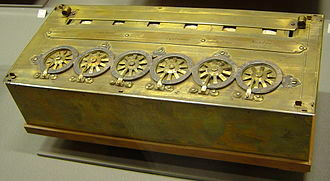
\includegraphics[width=0.9\linewidth]{image/pascaline.png}\end{center}
\end{multicols}

\noindent\rule{\linewidth}{.25mm}

\begin{multicols}{2}\setlength{\columnseprule}{.25mm}
\subsubsection{Document 2 : Le métier Jacquard}
Au début du \emph{XIX$^e$ siècle}, Joseph-Marie \emph{Jacquard} invente une machine à tisser mécanique capable de produire des tissus présentant des motifs complexes, en suivant des instructions contenues dans des cartes perforées défilant dans la machine.
\begin{center}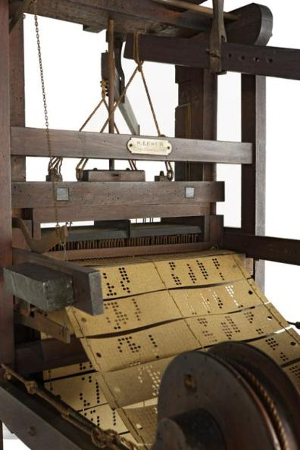
\includegraphics[width=0.9\linewidth]{image/metierJacquard1.jpg}\end{center}
\columnbreak
\subsubsection{Document 3 : La machine analytique de Babage}
Afin d'aider les marins lors de leur navigation, \emph{Babbage} envisage en 1822 de créer une machine qui produise une feuille de route en calculant la carte du ciel jour après jour pour les semaines à venir. Il réalise en \emph{1834}, qu'il peut créer une machine plus performante, capable d'exécuter n'importe quelle tâche qui pourrait lui être décrite. Inspiré par le métier à tisser Jacquard, il envisage que cette description, qui n'est qu'une suite de calculs, soit réalisée par des cartes perforées. Cette machine ne sera jamais finalisée.
\begin{center}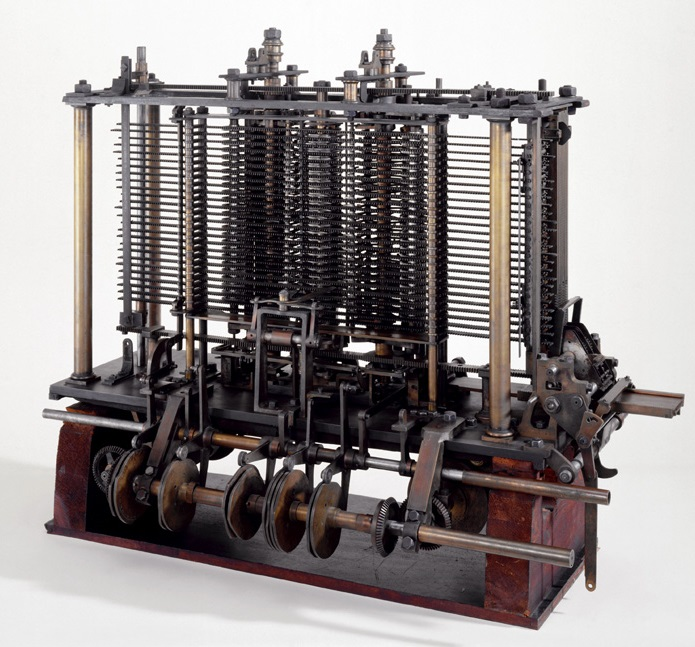
\includegraphics[width=\linewidth]{image/machine-analytique.jpg}\end{center}
\end{multicols}

\noindent\rule{\linewidth}{.25mm}

\begin{multicols}{2}
\subsubsection{Document 4 : Les cartes perforées}
Elles existeront jusqu'à la \emph{fin des années 1970}. Elles présentent l'énorme avantage de dissocier le temps d'écriture de l'information et le temps de sa lecture. Standardisée par la société IBM, les \emph{cartes perforées} présentent alors 80 colonnes et 12 lignes. Chaque colonne code, en binaire (0 ou 1), un caractère.
\columnbreak
\begin{center}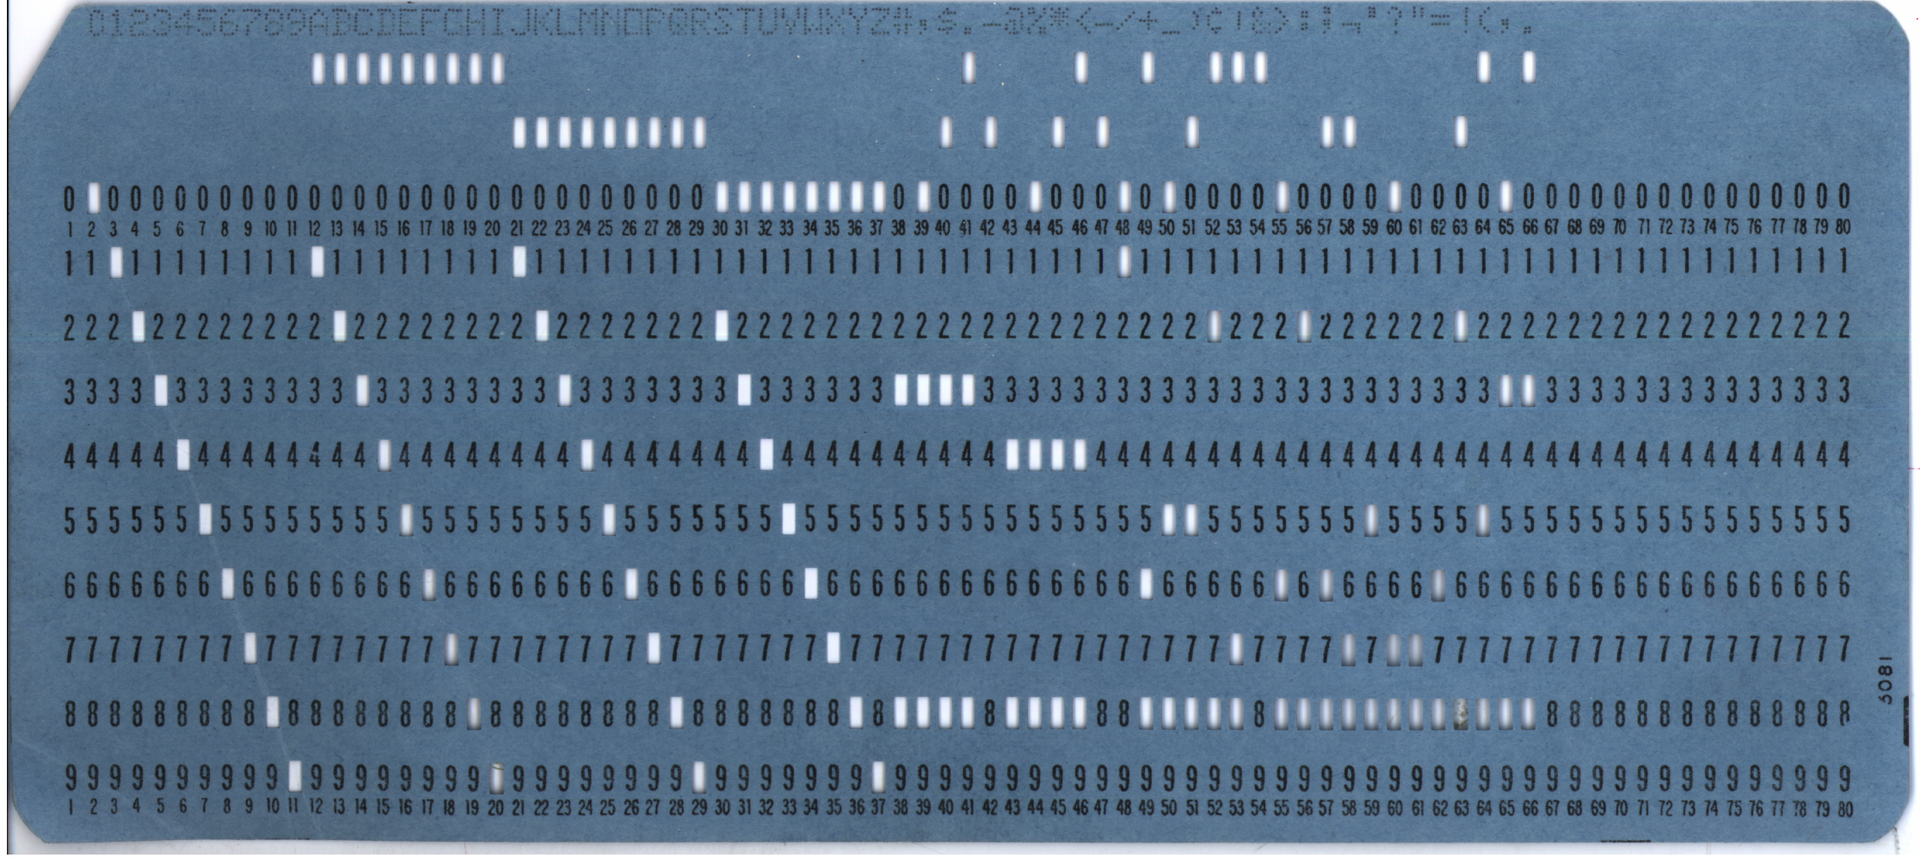
\includegraphics[width=0.9\linewidth]{image/Blue-punch-card-front-horiz.png}\end{center}
\end{multicols}

\section{Les précurseurs de la programmation}

\subsection{Ada Lovelace}

Ada Lovelace (1815-1852) est la fille du poète anglais Lord Byron. En 1833, elle rencontre Charles Babbage, qui est notamment l'inventeur d'une machine à calculer programmable connue sous le nom de machine analytique. Ada Lovelace traduit en anglais un article écrit en français sur la machine analytique de Babbage. Elle complète cet article de commentaires qui formalisent les idées de Babbage. 

Dans sa note A, elle promet que la machine sera capable de calculs abstrait. Elle entrevoit que de telles machines ne seront pas limitées à des calculs numériques mais pourront réaliser des opérations sur toute sorte d'objets. Elle ajoute qu'un jour, elles pourrait même composer de la musique.

Ada Lovelace commence sa Note G en affirmant que, malgré ses pouvoirs impressionnants, on ne peut pas vraiment dire que la Machine Analytique << pense >>. Cette partie de Note G est ce que Alan Turing appellera plus tard << l'objection de Lady Lovelace >>. Néanmoins, poursuit Lovelace, la machine peut faire des choses extraordinaires. Pour illustrer sa capacité à gérer des problèmes encore plus complexes, Lovelace fournit son programme de calcul des nombres de Bernoulli.

\subsubsection{Les nombres de Bernoulli}

Les nombres de Bernoulli $(B_n)$ peuvent être calculés de proche en proche en résolvant les équations suivantes, écrites à partir du triangle de Pascal. (Il y a un décalage entre la notation moderne et celle utilisé dans le document, que l'on prend comme référence ici)

\begin{multicols}{2}

Triangle de Pascal

\begin{tabular}{cccccccc}
$1$& $1$&     &     &     &    &    &\\
$1$& $2$&  $1$&     &     &    &    &\\
$1$& $3$&  $3$&  $1$&     &    &    &\\
$1$& $4$&  $6$&  $4$&  $1$&    &    &\\
$1$& $5$& $10$& $10$&  $5$& $1$&    &\\
$1$& $6$& $15$& $20$& $15$& $6$& $1$&\\
\prof{$1$}...& \prof{$7$}...&  \prof{$21$}...&  \prof{$35$}...&  \prof{$35$}...& \prof{$21$}...& \prof{$7$}...& \prof{$1$}...\\
\end{tabular}

Équations donnant $(B_n)$

(En notation moderne, il y a un premier terme avant $B_0$ égal à 1)

$\mathbf{1} + \mathbf{2}B_0 = 0$

$\mathbf{1} + \mathbf{3}B_0 + \mathbf{3}B_1 +  = 0$

$\mathbf{1} + \mathbf{4}B_0 + \mathbf{6}B_1 + \mathbf{4}B_2 = 0$

$\mathbf{1} + \mathbf{5}B_0 + \mathbf{10}B_1 + \mathbf{10}B_2 + \mathbf{5}B_3 = 0$

$\mathbf{1} + \mathbf{6}B_0 + \mathbf{15}B_1 + \mathbf{20}B_2 + \mathbf{15}B_3  + \mathbf{6}B_4= 0$

\prof{$\mathbf{1} + \mathbf{7}B_0 + \mathbf{35}B_1 + \mathbf{35}B_3  + \mathbf{21}B_4+ \mathbf{7}B_5= 0$}...
\end{multicols}


\begin{enumerate}
    \item Calculer :
    \begin{multicols}{6}
    $B_0=$\prof{$\frac{-1}{2}$}\pointsuite{1cm}
    
    $B_1=$\prof{$\frac{1}{6}$}\pointsuite{1cm}
    
    $B_2=$\prof{$0$}\pointsuite{1cm}
    
    $B_3=$\prof{$\frac{-1}{30}$}\pointsuite{1cm}
    
    $B_4=$\prof{$0$}\pointsuite{1cm}
    
    $B_5=$\prof{$\frac{1}{42}$}\pointsuite{1cm}
\end{multicols}

\item On remarque, et on peut démontrer que tous les termes d'indice pair sont nuls, sauf $B_0$ qui vaut $\frac{-1}{2}$. Le suivant non nul est donc $B_7$. Le programme proposé permet de le calculer (pour $n=4$). 

L'équation à résoudre est : $1 + \mathbf{9}B_0 + \mathbf{36}B_1 + \mathbf{126}B_3  + \mathbf{84}B_5  + \mathbf{9}B_7= 0$.

Elle est utilisée sous la forme $A_0 +A_1 B_1 + A_3 B_3  + A_5 B_5 + B_7 = 0$

\medskip
Quel devrait-être la valeur de $A_0$ ? $A_0 =$\prof{$A_0=\frac{1+9 B_0}{9}=(1-\frac{9}{2})\times\frac{1}{9}=\frac{-7}{2}\times\frac{1}{9}=\frac{-7}{18}$}\dotfill

\medskip
Vérifier que cela correspond à la formule $-\frac{1}{2}\frac{2n-1}{2n+1}=A_0$ pour $n=4$.\prof{$\frac{-1}{2}\frac{2\times4-1}{2\times4+1}=\frac{-1}{2}\frac{7}{9}=\frac{-7}{18}$}\dotfill


\medskip
\item Quels noms portent les variables utilisées ? \prof{$V_1$, $V_2$, $V_3$ (L'exposant gauche donne le nombre d'affectations.)}\dotfill


\medskip
\item Sont-elles initialisées ? (préciser) \prof{Les trois premières oui : à $1$, $2$ et $n$ (pour calculer $B_{2n-1}$)}\dotfill

\medskip
\item Quelles opérations sont utilisées ? \prof{(Seconde colonne) Les opérations $+$, $-$, $\times$ et $\div$.}\dotfill

\medskip
\item Lesquelles des instructions de base de la programmation sont utilisées (parmi l'affectation, les conditionnelles et les boucles) ? (Préciser)

\medskip\prof{L'affectation est utilisée à chaque étape (détaillée colonnes 4 et 5)}\dotfill

\medskip\prof{Les instructions conditionnelles ne sont pas explicitement utilisées.}\dotfill

\medskip\prof{Une boucle est clairement utilisée  : << Here follows a {\bfseries{repetition}} of ...>>}\dotfill

\medskip\prof{Il y a même des boucles imbriquées (les accolades en colonnes 1 et 2).}\dotfill

\end{enumerate}
En 1977, le département de la Défense des États Unis dénomme un langage de programmation Ada (inspiré du langage Pascal) en l’honneur d’Ada Lovelace. Ce langage, très structuré, est utilisé pour des projets nécessitant un très haut niveau
de fiabilité (domaines militaire, aéronautique, etc).

\newpage
\begin{tikzpicture}[remember picture, overlay]\node[]at(current page.center){\rotatebox{90}{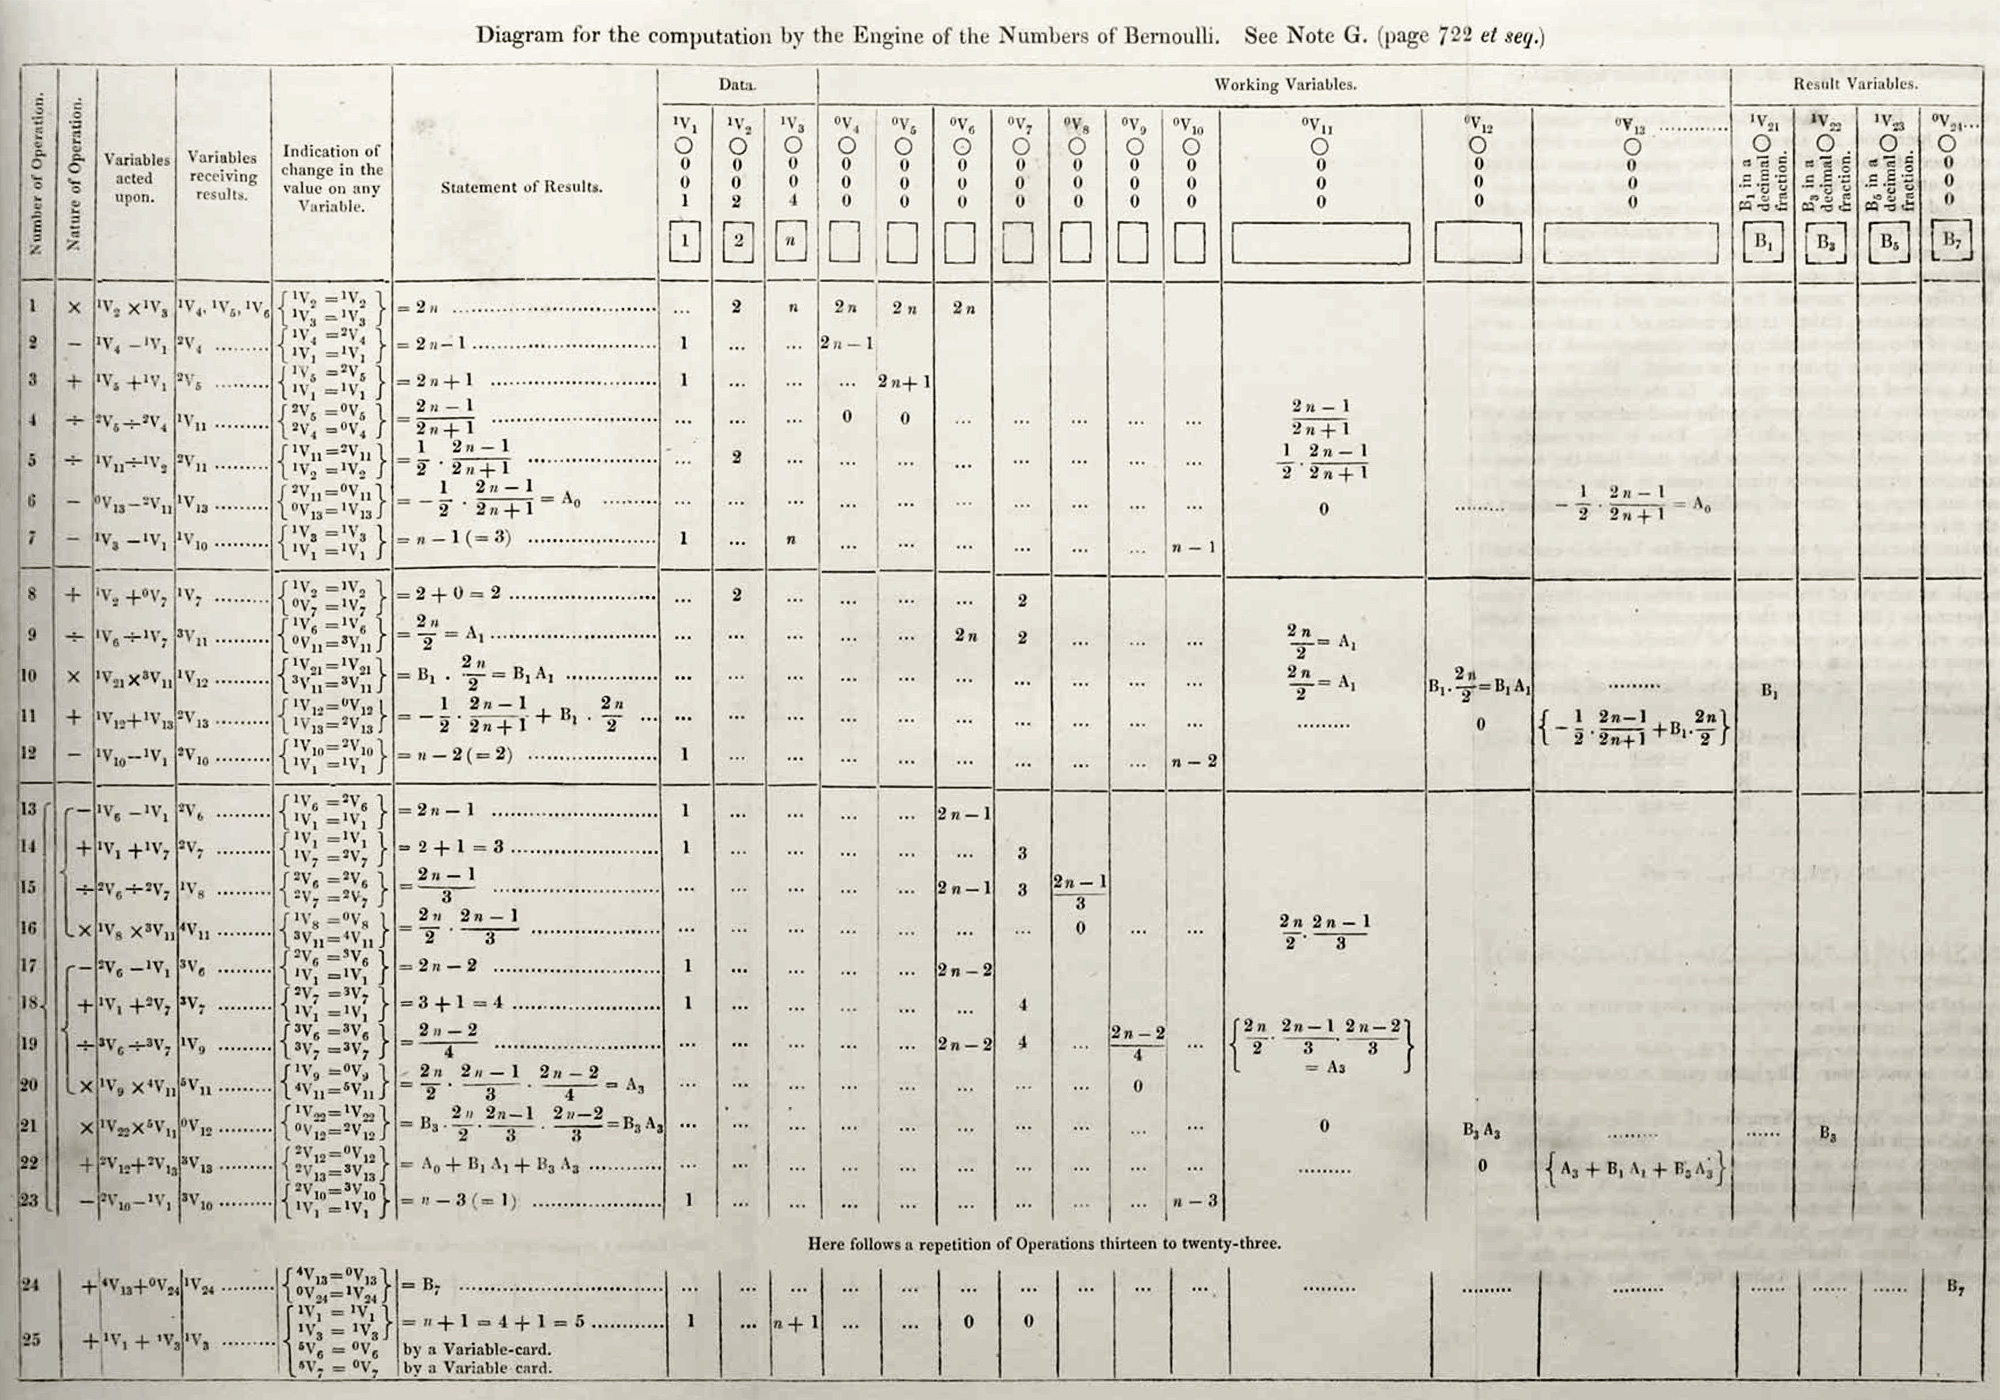
\includegraphics[scale=0.42]{image/Diagram_for_the_computation_of_Bernoulli_numbers.jpg}}};\end{tikzpicture}
~
\newpage
\subsection{Alan Turing}
En 1936, le mathématicien et cryptologue, Alan Turing a imaginé un modèle abstrait pour définir une notion qui jusqu'alors était restée intuitive : la calculabilité. Il cherche à définir la différence entre ce qui est calculable et ce qui ne l'est pas. Ce qui est calculable doit pouvoir peut se décomposer en un nombre fini d'étapes, pouvant être réalisées par une machine. 

Il imagine alors le moyen pour une machine de reproduire certaines actions humaines :

<< je fais le pari que d'ici 50 ans, une personne non prévenue n'aura plus le moyen de distinguer les réponses données par un ordinateur de celles données par un humain, et ce, sur n'importe quel sujet. >>

Cette machine se décrit très simplement. Elle utilise un ruban qui contient une suite de cases dans lesquelles sont inscrites des données (0 et 1). La machine est capable de lire ce qu'il y a dans les cases, de se déplacer sur le ruban d'une case à gauche ou à droite et d'écrire dans une case.

Ce modèle est aujourd'hui connu sous le nom de machine de Turing et est toujours utilisé en informatique théorique pour résoudre les problèmes de calculabilité. 

\begin{center}\href{https://videotheque.cnrs.fr/index.php?id_doc=3001&urlaction=doc}{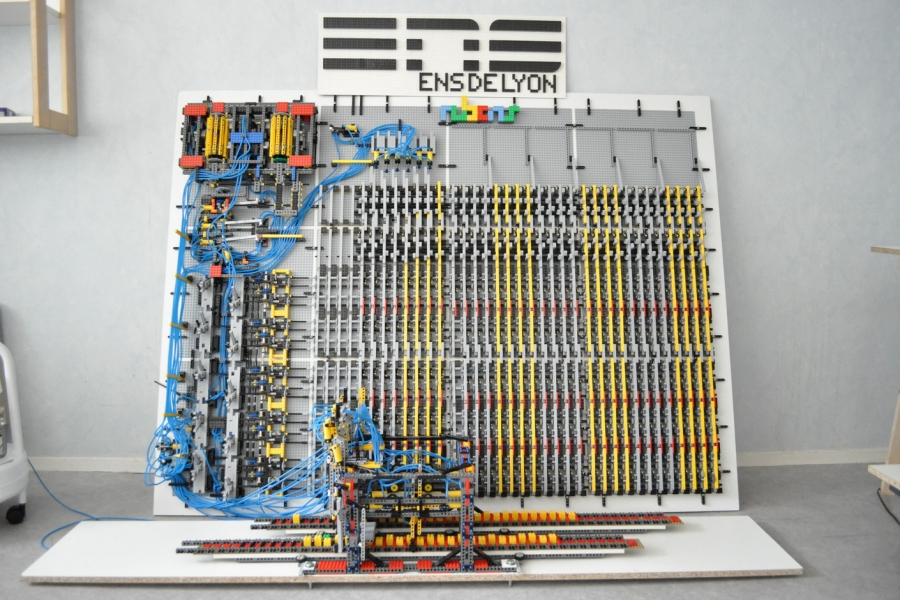
\includegraphics[width=0.9\linewidth]{image/Lego_Turing_Machine.jpg}}\end{center}

\subsection{Von Neumann}
En s'inspirant de ses prédécesseurs, il élabore en 1945, la première description d'un ordinateur dont le programme est stocké dans sa mémoire : ici, l'ordinateur dispose d'un processeur pour exécuter les instructions et d'une structure de stockage unique (Mémoire vive RAM) pour conserver à la fois les instructions et les données demandées ou
produite par le calcul. C'est le premier modèle de calculateur universel programmable concret dont le premier modèle sera commercialisé en 1951.

\begin{enumerate}
    \item Montrer (en utilisant tous les documents de ce cours) comment les avancées technologiques se sont construites en utilisant les technologies antérieurs.
    
    \medskip \prof{La première machine à calculer, la pascaline et les cartes perforées du métier Jacquard sont les bases de la machine}\dotfill
    
    \medskip \prof{analytique de Babage. C'est en en faisant la traduction qu'Ada Lovelace posa les bases de la programmation et initia}\dotfill
    
    \medskip \prof{la notion de machine universelle. Alan Turing formalisa la notion et Van Neumann en fit une description contrête.}\dotfill
    \item Expliquer pourquoi Alan Turing peut être considéré comme le père de l'intelligence artificielle.
    
    \medskip \prof{Alan Turing décrit ce qui est << calculable >> et prévoit que son modèle de machine, basé uniquement sur le calcul binaire}\dotfill
    
    \medskip \prof{ sera capable à terme de soutenir une conversation avec un humain sur n'importe quel sujet (sans que celui-ci ne devine}\dotfill
    
    \medskip\prof{ qu'il parle avec une machine).}\dotfill
\end{enumerate}

\section{Les ordinateurs autour de nous}

Expliquer en quoi les objets ci-dessous, de la vie courante, sont des ordinateurs et indiquer par qui ils sont programmables :
\begin{enumerate}
\begin{multicols}{2}
    \item Thermostat d'ambiance
    \begin{center}
    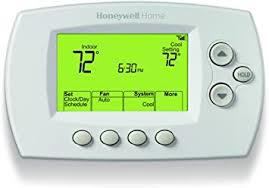
\includegraphics[height=9em]{image/thermostat.png}
    \end{center}
    \item Smartphone
    \begin{center}
    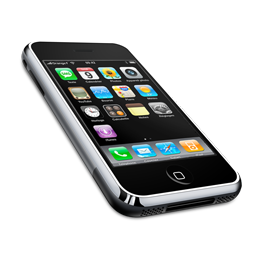
\includegraphics[height=9em]{image/smartphone.png}
    \end{center}
    \item Box internet
    \begin{center}
    \includegraphics[height=9em]{image/livebox.png}
    \end{center}
    \item Ordinateur de bord d'une voiture
    \begin{center}
    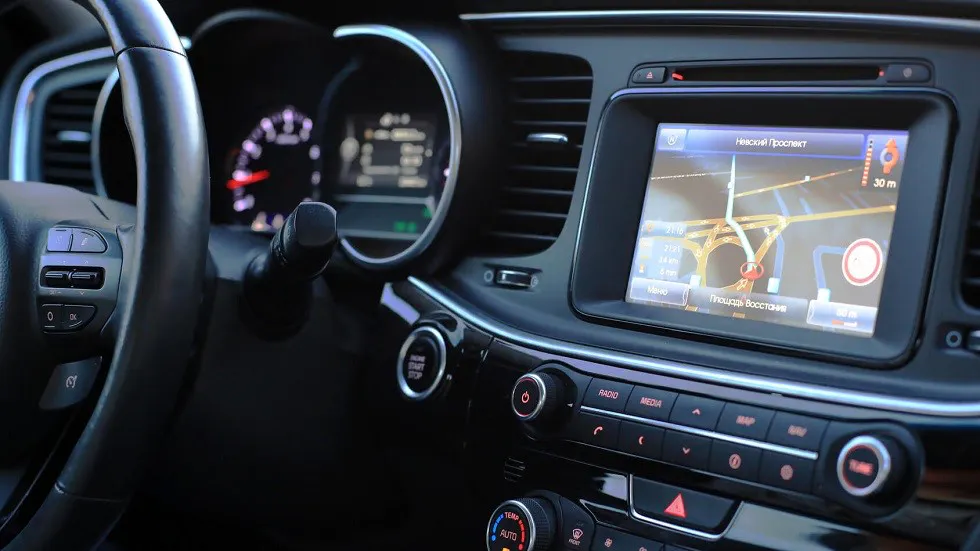
\includegraphics[height=9em]{image/ordinateurDeBord.png}
    \end{center}
\end{multicols}
    
    \medskip\prof{Tous les appareils cités possèdent un ou plusieurs processeurs et au minimum des boutons (entrées) et un écran (sortie).}\dotfill
    
    \medskip \prof{Il possèdent également tous une mémoire (au minimum pour stocker les réglages de l'utilisateur). }\dotfill
    
    \medskip \prof{Le thermostat d'ambiance est programmable/configurable par l'utilisateur (règlage de la température selon les heures).}\dotfill
    
    \medskip \prof{Le smartphone est programmable par l'utilisateur (averti) qui peut (télécharger et) installer des programmes écrits par des professionnels.}\dotfill 
    
    \medskip\prof{La box internet est programmable par le fournisseur d'accès et configurable par l'utilisateur.}\dotfill
    
    \medskip\prof{L'ordinateur de bord d'une voiture est programmable par le constructeur.}\dotfill
\end{enumerate}

\chapter{Numérisation de l'information}

Pour qu'une machine puisse opérer de manière automatique sur des informations, une première étape consiste à les numériser. On transforme ainsi sous forme de suites de nombres, les textes, les sons, les images et les vidéos. Les programmes eux-même, ne sont pour une machine que des données à traiter. On peut se donner une bonne image de la programmation de bas niveau (langage machine et assembleur) avec l'émulateur \href{http://www.peterhigginson.co.uk/RISC/}{http://www.peterhigginson.co.uk/RISC/} (\texttt{SELECT > add} puis \texttt{RUN} par exemple)

\section{Le système binaire}

Comme les cartes perforées des premiers calculateurs qui ne contenaient que des informations binaires : un trou ou pas, les ordinateurs modernes ne manipulent toujours que des informations binaires : une tension électrique ou pas. Formellement, on note \texttt{1} ou \texttt{0} ces deux informations et on appelle \emph{bit} : << \underline{Bi}nary dig\underline{it} >> ce plus petit élément d'information qui ne peut donc prendre que deux valeurs.

\subsection{Numération}
On apprend à l'école comment écrire un nombre en base 10, c'est à dire en utilisant les chiffres 0, 1, 2, 3, 4, 5, 6, 7, 8 et 9, en les positionnant de droite à gauche (unités, dizaines, centaines, milliers, ...). De la même façon, on peut les écrire en base 2, c'est à dire en utilisant les chiffres 0 et 1, en les positionnant de droite à gauche (unité, << deuzaine >>, ...) :

\begin{exemple*}{}{}
Pour compter le nombre d'étoiles ci-dessous :

\begin{center}
$\star\star\star\star\star\star\star\star\star\star\star\star\star$
\end{center}

On peut faire des paquets de 10 :

\begin{center}\begin{tabular}{c|c|c|c}
$10^3=1000$ & $10^2=100$ & $10$ & $1$ \\
\tikz\node{~}; & \tikz\node{~}; & \tikz\node[draw]{$\star\star\star\star\star\star\star\star\star\star$}; & \tikz\node{$\star\star\star$};\\
\end{tabular}

Il y a \texttt{0} paquet de 1000, \texttt{0} paquet de 100, \texttt{1} paquet de 10 et \texttt{3}  étoiles : \texttt{13} en décimal.
\end{center}

On peut aussi faire des paquets de 2 :

\begin{center}\begin{tabular}{c|c|c|c}
$2^3=8$ & $2^2=4$ & $2$ & $1$ \\
\tikz\node[draw]{\tikz\node[draw]{\tikz\node[draw]{$\star \star$}; \tikz\node[draw]{$\star \star$};}; \tikz\node[draw]{\tikz\node[draw]{$\star \star$}; \tikz\node[draw]{$\star \star$};};}; & \tikz\node{\tikz\node[draw]{\tikz\node[draw]{$\star \star$}; \tikz\node[draw]{$\star \star$};};}; & \tikz\node{\tikz\node{\tikz\node{~};};}; & \tikz\node{\tikz\node{\tikz\node{$\star$};};};\\
\end{tabular}

Il y a \texttt{1} paquet de 8, \texttt{1} paquet de 4, \texttt{0} paquet de 2 et \texttt{1}  étoiles : \texttt{1101} en binaire.
\end{center}

(Les Shadoks font des paquets de 4 - \href{https://www.youtube.com/watch?v=9bNZjP1LsNA&list=RDtpD0Pdr7oD0&index=1}{épisode 44 de la saison 2 de « Et voilà les Shadoks » de 1969})
\end{exemple*}

\begin{enumerate}
    \item Déterminer l'écriture binaire du nombre dont l'écriture décimal est : 228. (Préciser votre démarche.)
    
    \medskip\prof{On cherche à décrire 228 avec une succession de \texttt{1} et \texttt{0} correspondant à des puissances de 2 dans 228.}\dotfill
    
    \medskip\prof{On cherche la plus grande inférieure à 288 : 1, 2, 4, 8, 16, 32, 64, \underline{128}, 256. C'est $\text{128}=\text{2}^\text{7}$}\dotfill
    
    \medskip\prof{Alors $\text{228} = \text{128} + \text{100}$. Et on recommence avec 100 : jusqu'à $\text{228} = \text{128} + \text{64} + \text{32} + \text{4} = \texttt{11100100}_2$}\dotfill

    \item Retrouver l'écriture décimale du nombre binaire \texttt{10010010111}
    
    \medskip\prof{$\texttt{10010010111} = \text{2}^\text{10} + \text{2}^\text{7} + \text{2}^\text{4} + \text{2}^\text{2} + \text{2} + \text{1}$}\dotfill
    
    \medskip\prof{$\phantom{\texttt{10010010111}} = \text{1024} + \text{128} + \text{16} + \text{4} + \text{2} + \text{1} = \text{1175}$}\dotfill
\end{enumerate}

\subsection{Octet}

Un octet est une séquence de 8 bits. En anglais, octet se dit << Byte >> ($\neq$ << bit >>).

\begin{enumerate}
    \item Pourquoi le nombre 228 est-il codable sur un octet ? \prof{Il s'écrit en binaire avec 8 chiffres}\dotfill
    
     \medskip
    \item Quel est le plus grand entier codable sur un octet ? \prof{$\texttt{11111111}_2 = \texttt{100000000}_2 - \texttt{1}_1 = \text{256}-\text{1}=\text{255}$}\dotfill
    
     \medskip
    \item Combien d'informations distinctes sont codables sur un octet ? \prof{$\text{2}^\text{8} = \text{256}$ (c'est à dire de 0 à 255).}\dotfill
\end{enumerate}

\section{Le codage ASCII}

Le code ASCII (<< American Standard Code for Information Interchange>>) fait son apparition dans les années 1960. Son objectif était de standardiser le codage des caractères. À l'époque les informations se codaient sur 1 octet (contre 8 de nos jour sur des sytèmes dit << 32 bits >>). Mais un bit de cet octet était requis pour contrôler sa transmission. La table ASCII définissait donc 128 caractères (sur 7 bits).

\begin{exemple*}{Codage ASCII des lettres}
\begin{center}\begin{tabular}{ccccccccccc}
lettre & A& B& C& D& E& F& G& H& ... & Z \\
code & 65& 66& 67& 68& 69& 70& 71& 72& ... & 90 \\
\end{tabular}

~

\begin{tabular}{ccccccccccc}
lettre & a& b& c& d& e& f& g& h& ... & z \\
code & 97& 98& 99& 100& 101& 102& 103& 104& ... & 122 \\
\end{tabular}
\end{center}
\end{exemple*}

En général les langages de programmations donnent des fonctions permettant de coder ou de décoder en ASCII. (\texttt{CODE} et \texttt{CAR} avec un tableur, \mintinline{python3}{ord} et \mintinline{python3}{chr} en Python...)

\begin{exemple*}{Fonctions de codage}
\begin{multicols}{2}
\begin{center}
{\bfseries Avec un tableur}

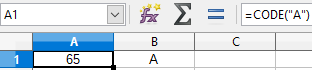
\includegraphics[width=0.9\linewidth]{image/codeA.png}

~

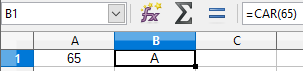
\includegraphics[width=0.9\linewidth]{image/car65.png}

~

{\bfseries Avec le langage Python}

\begin{console}
>>> ord('A')
65
>>> chr(65)
'A'
\end{console}
\end{center}
\end{multicols}
\end{exemple*}

(À faire à la maison)

\begin{enumerate}
    \item Quels sont les caractères codés entre le \texttt{'Z'} et le \texttt{'a'} ? (Détailler votre méthode.)
    
    \medskip\prof{\mintinline{python}{>>> for k in range(91,97):}}\dotfill
    
    \medskip\prof{\qquad\qquad\mintinline{python}{print(k,chr(k),end=' ')}}\dotfill
    
    \medskip\prof{\mintinline{python}{91 [ 92 \ 93 ] 94 ^ 95 _ 96 }~\texttt{`}}\dotfill
    
    \item Vérifier que l'écriture binaire des codes des lettres majuscules et minuscules ne diffère que d'un bit. Lequel ? (Détailler votre méthode.)
    
    \medskip\prof{De A à Z les codes vont  de 65 =  $\texttt{1000001}_2$ à 90 =  $\texttt{1011010}_2$}\dotfill
    
    \medskip\prof{De a à z les codes vont  de 97 =  $\texttt{1100001}_2$ à 122 =  $\texttt{1111010}_2$}\dotfill
    
    \medskip\prof{On passe donc d'une majuscule à une minuscule en changeant le bit de poids 5 uniquement}\dotfill
    
    \medskip\prof{Autre approche possible : 97 $-$ 65 $=$ 98 $-$ 66 $=$ ... $=$ 122 $-$ 90 $=$ 32 $=$ 2$^\text{5}$ ...}\dotfill
\end{enumerate}

\subsection{Art ASCII}
Le codage ASCII à inspiré les programmeurs puis les artistes depuis les années 1960. Ils en ont fait un art qui consiste à produire des images à l'aide des glyphes des caractères. 
\begin{multicols}{2}
La forme la plus simple d'art ASCII est la combinaison de deux ou trois caractères pour exprimer une émotion en texte : 

\begin{center}
\begin{tabular}{ccc}
\texttt{:)} & \texttt{:(} & \texttt{:'(} \\
sourire & triste & pleure \\
 \texttt{;)} & \texttt{:D} & \texttt{:p} \\
 clin d'œil  & rire & tire la langue \\
\end{tabular}
\end{center}

Un exemple plus complexe ci-contre.


\begin{center}
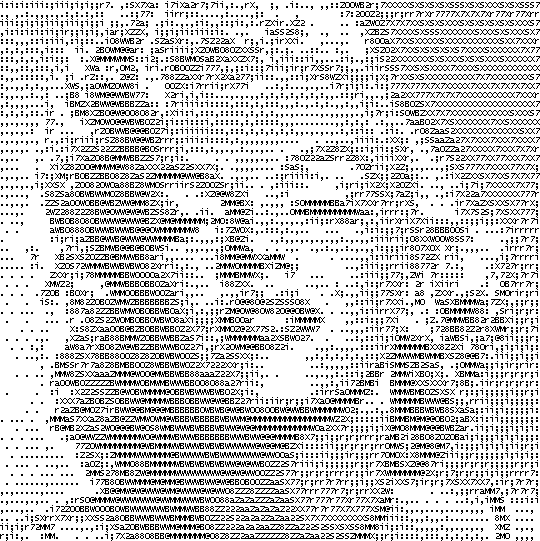
\includegraphics[height=5cm]{image/ASCII_Art_Marilyn_Monroe.png}
\end{center}
\end{multicols}
\section{Le codage d'une image}

Il suffit de quelques carrés noirs ou blancs pour représenter quelque chose. Avec une grille de 5 par 5, on peut par exemple suggérer les pièces d'un jeu d'échec :

\newcounter{x}\newcounter{y}
\begin{center}
\begin{tikzpicture}[scale=0.4]
\setcounter{x}{0}\setcounter{y}{0}
\foreach \k in {
  0,1,1,1,0,
  1,1,1,1,1, 
  1,1,1,1,1,
  0,1,1,1,0,
  1,1,1,1,1} {
    \ifnum\k=1{\fill(\thex cm,-\they cm)rectangle++(1,-1);}\fi
    \stepcounter{x}
    \ifnum\thex=5{\stepcounter{y}\setcounter{x}{0}}\fi
}
\draw [very thick, black!50, step=1.0cm] (0,-5) grid (5,0);
\end{tikzpicture} \quad
\begin{tikzpicture}[scale=0.4]
\setcounter{x}{0}\setcounter{y}{0}
\foreach \k in {
  1,0,1,0,1,
  1,1,1,1,1, 
  1,1,1,1,1,
  0,1,1,1,0,
  1,1,1,1,1} {
    \ifnum\k=1{\fill(\thex cm,-\they cm)rectangle++(1,-1);}\fi
    \stepcounter{x}
    \ifnum\thex=5{\stepcounter{y}\setcounter{x}{0}}\fi
}
\draw [very thick, black!50, step=1.0cm] (0,-5) grid (5,0);
\end{tikzpicture} \quad
\begin{tikzpicture}[scale=0.4]
\setcounter{x}{0}\setcounter{y}{0}
\foreach \k in {
  0,0,1,1,0,
  0,1,1,1,1, 
  1,0,1,1,1,
  0,1,1,1,0,
  1,1,1,1,1} {
    \ifnum\k=1{\fill(\thex cm,-\they cm)rectangle++(1,-1);}\fi
    \stepcounter{x}
    \ifnum\thex=5{\stepcounter{y}\setcounter{x}{0}}\fi
}
\draw [very thick, black!50, step=1.0cm] (0,-5) grid (5,0);
\end{tikzpicture} \quad
\begin{tikzpicture}[scale=0.4]
\setcounter{x}{0}\setcounter{y}{0}
\foreach \k in {
  0,0,1,0,0,
  0,0,1,1,0, 
  1,1,0,1,1,
  0,1,1,1,0,
  1,1,1,1,1} {
    \ifnum\k=1{\fill(\thex cm,-\they cm)rectangle++(1,-1);}\fi
    \stepcounter{x}
    \ifnum\thex=5{\stepcounter{y}\setcounter{x}{0}}\fi
}
\draw [very thick, black!50, step=1.0cm] (0,-5) grid (5,0);
\end{tikzpicture} \quad
\begin{tikzpicture}[scale=0.4]
\setcounter{x}{0}\setcounter{y}{0}
\foreach \k in {
  0,0,1,0,0,
  1,1,1,1,1, 
  1,1,1,1,1,
  0,1,1,1,0,
  1,1,1,1,1} {
    \ifnum\k=1{\fill(\thex cm,-\they cm)rectangle++(1,-1);}\fi
    \stepcounter{x}
    \ifnum\thex=5{\stepcounter{y}\setcounter{x}{0}}\fi
}
\draw [very thick, black!50, step=1.0cm] (0,-5) grid (5,0);
\end{tikzpicture} \quad
\begin{tikzpicture}[scale=0.4]
\setcounter{x}{0}\setcounter{y}{0}
\foreach \k in {
  0,0,1,0,0,
  0,1,1,1,0, 
  0,0,1,0,0,
  0,1,1,1,0,
  1,1,1,1,1} {
    \ifnum\k=1{\fill(\thex cm,-\they cm)rectangle++(1,-1);}\fi
    \stepcounter{x}
    \ifnum\thex=5{\stepcounter{y}\setcounter{x}{0}}\fi
}
\draw [very thick, black!50, step=1.0cm] (0,-5) grid (5,0);
\end{tikzpicture}
\end{center}

On appelle \emph{pixel} (pour << {\bfseries pi}cture {\bfseries el}ement >> chacune de ces cases et les premières technologies codaient \texttt{0} une case blanche et \texttt{1} une case noire.

\begin{multicols}{2}
\begin{enumerate}
   \item Proposer un codage de l'image ci-contre inspirée de Space invaders (Shoot'em up de 1978)
   
   \medskip\prof{\texttt{01110 10101 11111 01010 10101}}\dotfill
   
   ~
   \begin{center}\begin{tikzpicture}[scale=0.4]
\setcounter{x}{0}\setcounter{y}{0}
\foreach \k in {
  0,1,1,1,0,
  1,0,1,0,1, 
  1,1,1,1,1,
  0,1,0,1,0,
  1,0,1,0,1} {
    \ifnum\k=1{\fill(\thex cm,-\they cm)rectangle++(1,-1);}\fi
    \stepcounter{x}
    \ifnum\thex=5{\stepcounter{y}\setcounter{x}{0}}\fi
}
\draw [very thick, black!50, step=1.0cm] (0,-5) grid (5,0);
\end{tikzpicture}
\end{center}
\end{enumerate}
   \end{multicols}
   \begin{multicols}{3}
   \begin{enumerate}\setcounter{enumi}{1}
   \item Noircir quelques carrés sur la figure ci-contre, écrire son code et le proposer à votre voisin. Trouver ce que représente son dessin à partir de son code.
   
   \begin{center}
   \begin{tikzpicture}[scale=0.4]
\draw [very thick, black!50, step=1.0cm] (0,-5) grid (5,0);
\end{tikzpicture}

\medskip\dotfill
   
   \begin{tikzpicture}[scale=0.4]
\draw [very thick, black!50, step=1.0cm] (0,-5) grid (5,0);
\end{tikzpicture}

\medskip\dotfill
\end{center}
\end{enumerate}
   \end{multicols}
   
   De nos jours chaque pixel n'est plus codé sur un seul bit, mais sur 24, répartis en 3 groupes de 8, chaque groupe représentant l'intensité lumineuse d'une couleur primaire : Rouge, Verte ou Bleue.
   
   \begin{enumerate}\setcounter{enumi}{2}
       \item Écrire le codage de la couleur (orange) sélectionnée ci-dessous :
       
       \begin{center}
       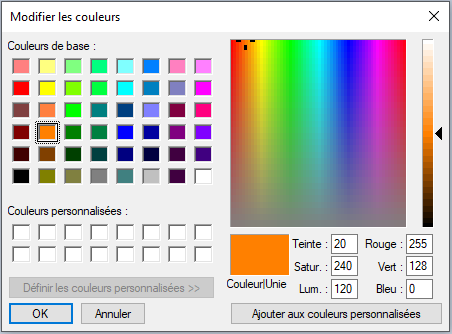
\includegraphics[scale=0.75]{image/rvborange.png}
       
       \medskip\prof{\texttt{1111 1111 1000 0000 0000 0000}}\dotfill
       \end{center}
       \item Proposer le codage d'un gris moyen :
       
       \medskip\prof{\texttt{1000 0000 1000 0000 1000 0000}}\dotfill
       
       
   \end{enumerate}
   
   \newpage
   
\section{Tailles et types de fichier}

\subsection{Ordres de grandeur}

On vient de voir comment on peut coder un nombre, comment on peut numériser une lettre donc un texte, donc un programme. On a également vu comment numériser une image. Les technologie de prise de vue ou de son permettent encore de numériser ce que l'on voit et ce que l'on entend. 

\begin{enumerate}
    \item Compléter les informations du tableau ci-dessous, donnant quelques valeurs élémentaires du traitement de l'information par un ordinateur.
    
    \begin{center}
    \begin{tabular}{|c|c|l|l|}\hline
    Information & \multicolumn{2}{c|}{Encodage}& Nombre de valeurs \\
    à numériser & en bit & en octet &   \\ \hline
    Texte (ASCII) & 8 & \rule{0pt}{1.5em}\prof{1} & \prof{256}\\ \hline
    Son (CD) & 16 & \rule{0pt}{1.5em}\prof{2} & \prof{65 536}\\ \hline
    Image (RVB) & 24 & \rule{0pt}{1.5em}\prof{3} & \prof{16 777 216} \\ \hline
    \end{tabular}
    \end{center}
    \item Sur le site \href{www.gutenberg.org}{www.gutenberg.org}, on trouve par exemple le roman << Notre-Dame de Paris >> de Victor Hugo. La version en texte contient \np{1117109} caractères.
\begin{enumerate}
        \item Sur combien de bits ; d'octets ; de mégaoctets est-il codé ?
        
    
        
        \medskip\prof{\np{1117109} octets $=$ \np{8936872} bits $\approx$ \np{1,1}Mo}\dotfill
        \item Sur le site sont proposés les chargements suivants :
        
\begin{center}
    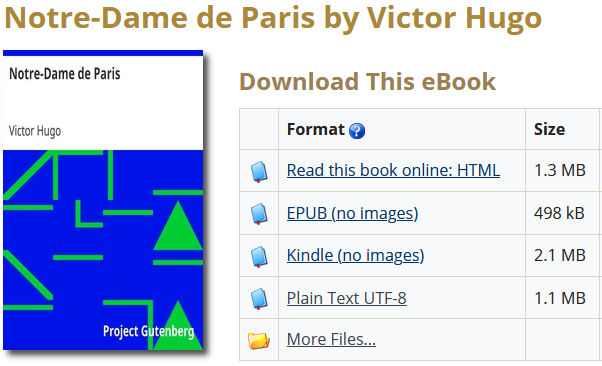
\includegraphics[scale=0.66]{image/vhugo.png}
\end{center}

        
        \begin{itemize}
            \item Que signifient << MB >>  et << kB >> ? \prof{MB pour MégaByte, donc Mo en français. kB pour kiloByte donc ko}\dotfill
            
            \medskip
            \item Pourquoi le fichier HTML est-il plus lourd ? \prof{Il faut rajouter les informations de structure de la page.}\dotfill
            
            \medskip
            \item Pourquoi le fichier EPUB est-il plus léger ? \prof{Il est compressé.}\dotfill
        \end{itemize}
    \end{enumerate}
    \item On considère un smartphone dont l'écran comporte \np{2560} pixels en largeur sur \np{1440} pixels en hauteur.
    
    \medskip
    \begin{enumerate}
        \item Combien l'écran contient-il de pixels ? \prof{\np{2560} $\times$ \np{1440} $=$ \np{3 686 400}}\dotfill
        \item Combien d'octets sont nécessaires pour enregistrer une capture d'écran ?
        
        \medskip \prof{\np{3 686 400} $\times$ \np{3} $=$ \np{11 059 200}. Soit $\approx$ 11 Mo}\dotfill
    \end{enumerate}
    \item Pour enregistrer un son échantillonner sur 16 bits à \np{44,1}kHz (\np{44100} fois par seconde) en stéréo.
    \begin{enumerate}
        \item Combien de bits d'informations sont enregistrées en une minute ?
        
        \medskip\prof{60 (secondes) $\times$ 44100 $\times$ 2 (stéréo) $\times$ 16 (bits) $=$ \np{84 672 000}. Soit \np{10,584}Mo.}\dotfill
        \item Combien de minutes d'enregistrement permet un CD de \np{550}Mo à cette qualité ? 
        
        \medskip\prof{550 $\div$ \np{10,584} $\approx$ \np{52} (minutes).}\dotfill
    \end{enumerate}
\end{enumerate}

\subsection{Extensions}

Pour un système d'exploitation, on peut distinguer deux grandes familles de fichiers informatiques :

\begin{itemize}
    \item Les fichiers de << {\bfseries données} >>. La plupart des informations qui se trouvent sur un disque dur sont sous la forme de fichiers de données (textes, images, ...). Chaque fichier est identifié par son nom suivi d'une extension qui permet au système d'exploitation de connaitre le programme à utiliser pour manipuler le fichier.
    \item Les fichiers << {\bfseries exécutables} >>. Sous Windows, par exemple, les fichiers exécutables sont ceux qui portent les extensions \texttt{.exe} ou {.com}.
\end{itemize}

\begin{exemple*}{Extensions de fichiers}
\begin{center}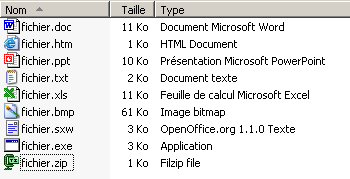
\includegraphics[scale=1]{image/extensions.png}\end{center}
\end{exemple*}

\medskip Citer au moins une extension possible pour chacun des types de fichiers suivants : 
    
    \begin{multicols}{5}
    Texte
    
    \prof{\texttt{.doc}, \texttt{.txt}}\dotfill   
     
    Son
    
    \prof{\texttt{.wav}, \texttt{.mp3}}\dotfill 
       
    Image
    
    \prof{\texttt{.bmp}, \texttt{.png}}\dotfill   
     
    Exécutable
    
    \prof{\texttt{.exe}, \texttt{.com}}\dotfill   
     
    Vidéo
    
    \prof{\texttt{.mp4}, \texttt{.avi}}\dotfill   
    \end{multicols}

\section{Les supports de stockage}

\begin{center}\begin{tikzpicture}
\draw[-latex](0,0)--(15.5,0);
\draw(0,2pt)node[above right]{1725}--(0,-1)node[right,yshift=1ex]{Carte perforée}node[below right=0pt,inner sep=0pt]{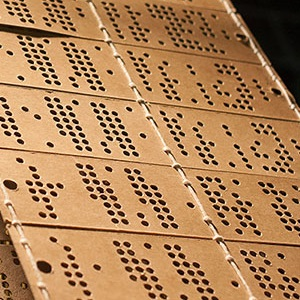
\includegraphics[width=2cm]{image/histoire/1725.jpg}};
\draw[line width=1pt,white,dashed](0.5,0)--(1,0);
\draw[line width=1pt,white](1,0)--(1.5,0);
\draw[line width=1pt,white,dashed](1.5,0)--(2,0);
\draw(2.5,2pt)node[above]{1890}--(2.5,-1)node[right,yshift=1ex]{Carte IBM}node(P)[below right=0pt,inner sep=0pt]{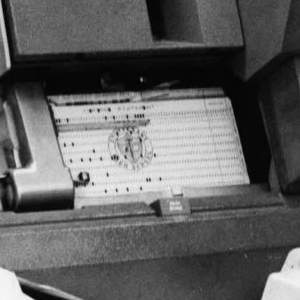
\includegraphics[width=2cm]{image/histoire/1890.png}};
\node[right=0.6cm]at(P.east){\cursive Support physique};
\draw[line width=1pt,white,dashed](3,0)--(3.5,0);
\draw[line width=1pt,white](3.5,0)--(4,0);
\draw[line width=1pt,white,dashed](4,0)--(4.5,0);
\draw(5.2,2pt)node[above]{1951}--(5.2,-4)node[right,yshift=2.5ex,text width=2cm]{Bandes\\ magnétiques}node(M)[below=0pt,inner sep=0pt]{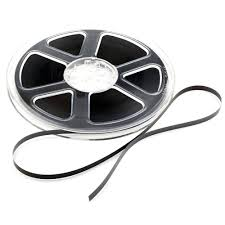
\includegraphics[width=2cm]{image/histoire/1951.jpg}};
\node[left,xshift=-1cm]at(M){\cursive Support magnétique};
\draw(7.5,2pt)node[above]{1971}--(7.5,-4)node[right,yshift=1ex]{Disquettes}node[below right=0pt,inner sep=0pt,xshift=-1.4cm]{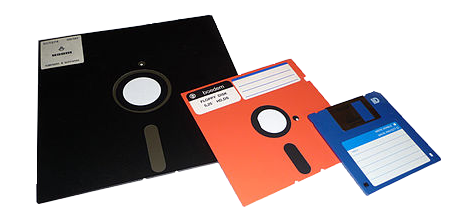
\includegraphics[height=2cm]{image/histoire/disquettes.png}};
\draw(9.7,2pt)node[above]{1982}--(9.7,-1)node[right=1pt,yshift=1ex]{CD}node[below,inner sep=0pt]{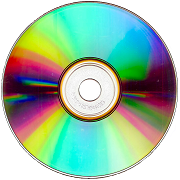
\includegraphics[height=2cm]{image/histoire/CD-ROM.png}};
\draw(12.3,2pt)node[below right, yshift=-4pt]{1995}--(12.3,-7)node[left, yshift=1ex]{SmartMedia}node(E)[below,inner sep=0pt]{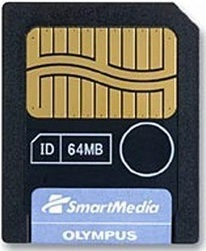
\includegraphics[height=1cm]{image/histoire/smartmedia.jpg}};
\node[left,xshift=-1cm]at(E){\cursive Support électronique};
\draw(12.1,2pt)node[above]{1994}--(12.1,-4)node[right=1pt,yshift=1ex]{ZIP}node[below,inner sep=0pt]{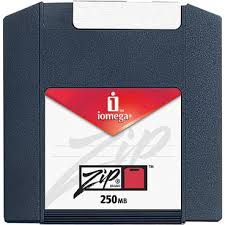
\includegraphics[height=2cm]{image/histoire/zip.jpg}};
\draw(13.1,2pt)node[above]{1999}--(13.1,-7)node[yshift=1ex]{SD}node[below,inner sep=0pt]{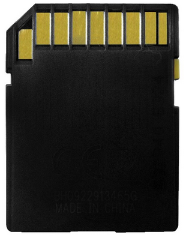
\includegraphics[height=1cm]{image/histoire/sd.png}};
\draw(12.3,-1)node[right=1pt,yshift=1ex]{DVD}node[below,inner sep=0pt]{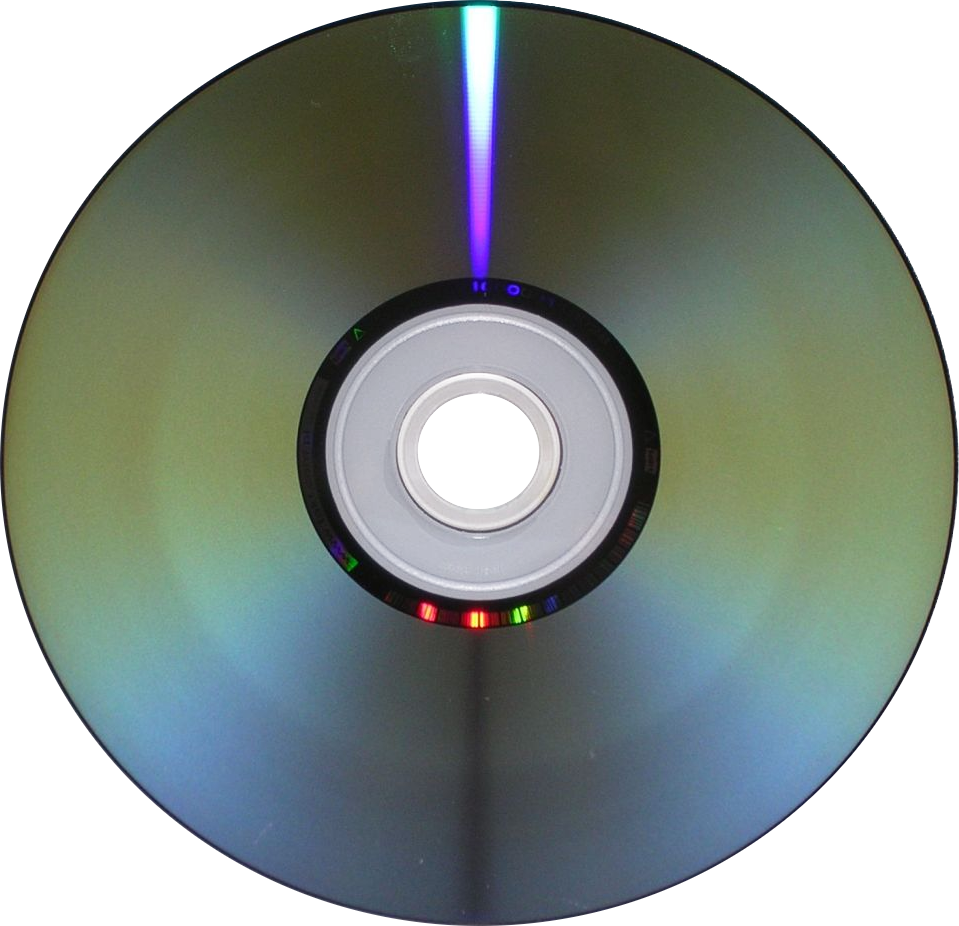
\includegraphics[height=2cm]{image/histoire/DVD.png}};
\draw(13.5,2pt)node[below right,yshift=-4pt]{2001}--(13.5,-7)node[right,yshift=1ex]{clé USB}node[below right,inner sep=0pt]{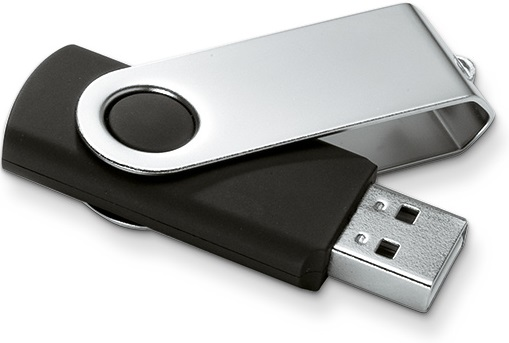
\includegraphics[height=1cm]{image/histoire/cleusb.jpg}};
\draw(14.7,2pt)node[above]{2006}--(14.7,-1)node[yshift=1ex]{Blu-ray}node[below,inner sep=0pt]{
\includegraphics[height=2cm]{image/histoire/blu-ray.png}};
\end{tikzpicture}\end{center}

\vspace{-0.75cm}
(Recherche à la maison)

Quelles étaient (sont) les capacités de stockage des supports suivants ?

\begin{multicols}{6}
 
 Carte IBM
 
 \medskip\prof{120 octets}\dotfill
 
 
 Disquette
 
 \medskip\prof{\np{1,44}Mo}\dotfill
 
 CD
 
 \medskip\prof{550 à 700 Mo}\dotfill
 
 DVD
 
 \medskip\prof{\np{4,7} à 17 Go}\dotfill
 
 Blu-Ray
 
 \medskip\prof{25 à 50 Go}\dotfill
 
 clé USB
 
 \medskip\prof{8 Mo à 256 Go...}\dotfill
\end{multicols}

\chapter{Programmation et bogue informatique}

Les programmes informatiques sont écrits par des opérateurs humains dans des langages sous forme de texte ou sous formes de graphiques. Ces programmes sont ensuite traduits en suite d'instructions qu'un processeur doit exécuter. Ils peuvent être stockés, transportés et traité par des ordinateurs.

Citer 5 langages informatiques.
    
    \medskip\prof{(Il y en a des centaines) (Fortran, Ada,) PHP, C\#, JavaScript, Java, Python}\dotfill
    
\medskip Il y a trois fondamentaux dans la programmation :

\begin{itemize}
    \item L'accès en lecture et/ou écriture à la mémoire. Cela peut se faire à l'aide de << variables >>
    \item Les branchements permettant de passer d'un partie du code à l'autre sous certaines conditions. Cela peut se faire à l'aide d'<< instructions conditionnelles >>.
    \item La répéter, autant que nécessaire, de certaines parties du code. Cela peut se faire à l'aide de << boucles >>.
\end{itemize}
    
\section{Bogue}

Un programme peut comporter jusqu'à plusieurs centaines de millions de lignes de code, ce qui rend très probable la présence d'erreurs appelées bogues. Ces erreurs peuvent conduire un programme à avoir un comportement inattendu et entraîner des conséquences graves.


\begin{multicols}{2}Le 9 septembre 1947, à l'université Harvard , le calculateur Mark II défaille : quelle est la source de la panne ? L'équipe de Grace Hopper (informaticienne, mathématicienne et officier supérieure de la marine américaine), chargée de l'appareil, lance ses investigations... Et découvre que c'est un insecte — << \pointsuite{1cm} >> en anglais — qui a provoqué un court-circuit dans les entrailles de l'ordinateur.

Après l'avoir découvert, grillé, entre les flancs du Mark II, l'équipe de Grace Hopper a décidé de scotcher la mite dans le journal de bord de l’ordinateur (le document est conservé au musée Smithsonian de Washington).

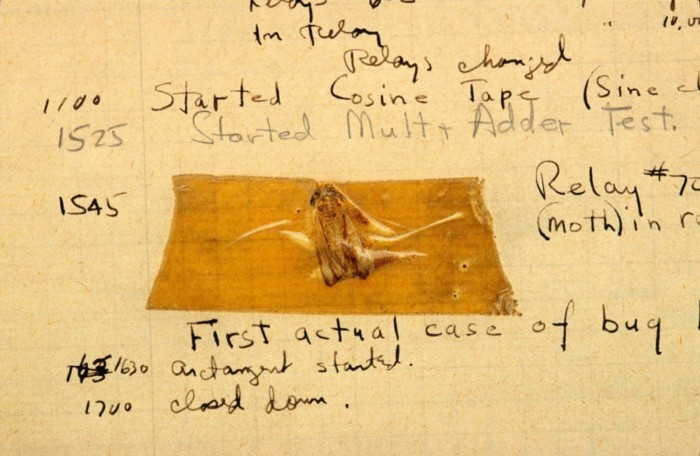
\includegraphics[width=\linewidth]{image/bug.jpg}
\end{multicols}

Pour comrendre ce qu'est réellement un bogue (ou bug) informatique, écouter la leçon inaugurale de Gérard Berry, au Collège de France, en 2008 : << Pourquoi et comment le monde devient numérique >> de 34min à 40min30

\href{https://www.college-de-france.fr/site/gerard-berry/inaugural-lecture-2008-01-17-18h00.htm}{https://www.college-de-france.fr/site/gerard-berry/inaugural-lecture-2008-01-17-18h00.htm}

Étude d'un cas : La fusée Ariane 5. (Documents page suivante.)

\begin{enumerate}
    \item Quelle a été la cause de l'explosion en vol de la fusée Ariane 5 en 1996 ?
    
    \medskip\dotfill
    
    \medskip\dotfill
    
    \item Quelles recommandations ont été faites pour éviter que l'accident ne se reproduise ?
    
    \medskip\dotfill
    
    \medskip\dotfill
\end{enumerate}

Un autres exemples explicités par Gérard Berry en 2019 : << Où va l'informatique ? >> de 1h39 à 1h48 :

\href{https://www.college-de-france.fr/site/gerard-berry/course-2019-01-23-16h00.htm}{https://www.college-de-france.fr/site/gerard-berry/course-2019-01-23-16h00.htm}

\begin{enumerate}[resume]
    \item Les bogues de contrôle moteur expliqués dans cette vidéo sont-ils très différents de ceux d'Ariane 5 ?
    
    \medskip\dotfill
    
    \medskip\dotfill
\end{enumerate}
\subsubsection{Document 1 : Explosion d'ariane 5.}

\begin{center}
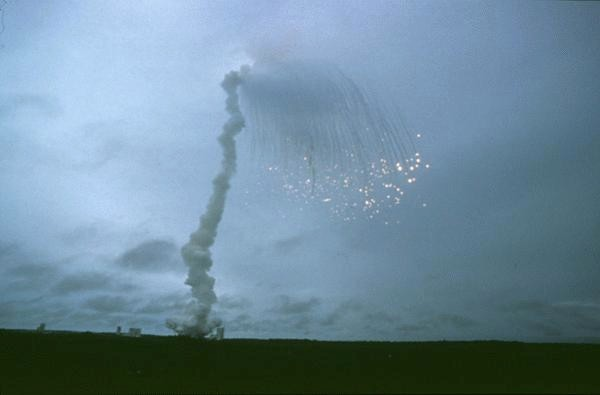
\includegraphics[scale=0.6]{image/ariane-v501-4juin96.jpg}

En vidéo : \href{https://www.youtube.com/watch?v=fCnO-UYF3co}{https://www.youtube.com/watch?v=fCnO-UYF3co}
\end{center}

\subsubsection{Document 2 : dans Libération le 24 juillet 1996 - Jean-Dominique Merchet.}

\begin{center}\fbox{\begin{minipage}{0.9\linewidth}L'explosion d'Ariane 5, le 4 juin, a été provoquée par une erreur de conception d'un logiciel informatique. C'est la conclusion à laquelle est arrivée la commission d'experts qui a rendu public son rapport, hier à Paris.

Concrètement, le logiciel n'a pas réussi à digérer certaines données concernant la << vitesse horizontale >> d'Ariane 5. Une fusée ne s'élève pas sur une trajectoire purement verticale; peu après le décollage, elle se penche légèrement. La vitesse à laquelle elle quitte la verticale de son point de lancement est sa << vitesse horizontale >>. Celle-ci << a dépassé une limite inscrite dans le logiciel du calculateur >>, affirment les rapporteurs de la commission présidée par Jacques-Louis Lions, de l'Académie des sciences.


<< Nous sommes tous coupables», a affirmé Jean-Marie Luton, directeur général de l'Agence spatiale européenne (ESA). Le système de référence inertielle SRI a déjà été utilisé à vingt-trois reprises lors des tirs d'Ariane 4. Mais << on >> a oublié que la trajectoire d'Ariane 5 n'était pas la même que celle de sa soeur... 

Au passage, les enquêteurs ont découvert d'autres << faiblesses éventuelles de conception au niveau du système de contrôle de vol >> et constaté << une anomalie >> au niveau de la pression hydraulique des vérins de la tuyère du moteur principal. Le coût des modifications et vérifications est évalué entre 2 et 4\% du coût du programme Ariane 5, c'est-à-dire une somme comprise entre 740 millions et 1,48 milliard de francs.
\end{minipage}}\end{center}

\subsubsection{Document 1 : Rapport de la commission d'enquête le 23 juin 1996.}

\begin{center}\fbox{\begin{minipage}{0.9\linewidth}
{\bfseries 3 CONCLUSIONS}

[...] Les revues et essais approfondis effectués dans le cadre du programme de développement d'Ariane 5 ne comportaient pas les analyses ou essais adéquats du système [...] qui auraient pu mettre en évidence la défaillance potentielle.

{\bfseries 4 RECOMMANDATIONS}

2- Mettre en place une installation d'essais qui réunisse, dans la mesure des possibilités techniques, un maximum d'équipements réels, introduire dans cette installation des données réalistes, et procéder à des essais complets en boucle fermée au niveau systèmes. Procéder à des simulations complètes avant toute mission. Étendre la couverture des essais.

11- Revoir la couverture des essais réalisés sur les équipements existants et l'étendre en cas de besoin.

12- Traiter les documents de justification avec autant d'attention que le code. Améliorer la technique visant à assurer la cohérence entre le code et ses justifications.
\end{minipage}}\end{center}

\section{Tests et corrections de programmes}

\subsection{Typage des variables}

En informatique, une variable est un espace mémoire identifié par un nom et pouvant être modifiée. Quand on modifie la mémoire correspondant à une variable, on dit que l'on affecte une valeur à la variable. 

\begin{multicols}{2}
Écriture algorithmique : \columnbreak

\begin{algorithm}[H]
\nonl $x \leftarrow 2$\;
\end{algorithm}
\end{multicols}

\begin{multicols}{2}
Programmation Python : \columnbreak

\begin{console}x = 2\end{console}
\end{multicols}


Cette valeur peut être la numérisation ne n'importe quelle information. Pour pouvoir décoder la mémoire correspondant à une variable, il faut donc savoir de quel genre d'information il s'agit : un entier naturel, relatif, un réel, un caractère, un pixel ? C'est ce que l'on appelle le {\bfseries type} de la variable.

\begin{exemple*}{Types de variables}
\begin{multicols}{4}\begin{center}
Entier

\begin{console}[escapeinside=||]
>>> type(1)
<class |\metastring{int}|>
\end{console}

\columnbreak

Réel

\begin{console}[escapeinside=||]
>>> type(1.0)
<class |\metastring{float}|>
\end{console}

\columnbreak


Chaine de caractères

\begin{console}[escapeinside=||]
>>> type('1.0')
<class |\metastring{str}|>
\end{console}

\columnbreak

Booléen

\begin{console}[escapeinside=||]
>>> type(True)
<class |\metastring{bool}|>
\end{console}
\end{center}
\end{multicols}
\end{exemple*}

\begin{multicols}{2}
On considère le programme Python ci-contre.

\begin{enumerate}
    \item Quel(s) test(s) pourrait-on mettre en place pour vérifier le comportement normal de ce programme ?
    
    \medskip\prof{Entrer 12; 18 ou 20}\dotfill
    
    \medskip\prof{Sortie attendue : Vous êtes mineur ; majeur ; majeur}\dotfill
\end{enumerate}

\begin{python}
age = input("Quel est votre âge ? ")
if age < 18 :
    print("Vous êtes mineur.")
else :
    print("Vous êtes majeur.")
\end{python}
\end{multicols}
\begin{enumerate}\setcounter{enumi}{1}
    \item Quelque soit l'entrée, le programme ne répond pas et affiche le message :
    
    \begin{console}
Traceback (most recent call last):
  File "C:\Users\Prof\Desktop\EnsSci\majeur.py", line 2, in <module>
    if age < 18 :
TypeError: '<' not supported between instances of 'str' and 'int'
\end{console}
Expliquer l'erreur :

\medskip\prof{Les valeurs entrées sont des chaines de caractères et ne peuvent donc pas être comparées à l'entier 18.}\dotfill

Comment la corriger ?

\medskip\prof{Il faut lire les cratères de la chaine pour en déduire un entier. Par exemple juste après la ligne 1 : \mintinline{python3}{age = int(age)}.}\dotfill
\item Proposer un autre test qui ferait encore boguer le programme. 

\medskip\prof{La modification \mintinline{python3}{age = int(age)} ne permet pas de prendre en compte une entrée non entière comme \np{12,5}.}\dotfill
\end{enumerate}

\bigskip

De manière générale, il peut être très difficile de tenir compte de toutes les entrées possibles d'un utilisateur. Il est parfois plus simple de laisser l'erreur se produire, de l'intercepter et de la traiter, par exemple en indiquant à l'utilisateur que la valeur entrée n'est pas conforme.

\medskip
Mettre en place un jeu de tests le plus exhaustif possible n'est par ailleurs pas suffisant pour prouver qu'un programme n'est pas boguer. Des preuves plus formelles (et plus complexes à mettre en place) existent.

\newpage
\subsection{Instructions conditionnelles}

\subsubsection{Radar automatique}

Sur autoroute, la vitesse pour les véhicules légers (VL) est limitée à 130 km.h$^{-1}$ et pour les poids lourds (PL) à 90 km.h$^{-1}$. Un radar possède au moins 2 capteurs permettant de mesurer la vitesse et la hauteur des véhicules circulant sur l'autoroute.

\begin{multicols}{2}

On propose le programme suivant :

\begin{python}
def Amende(h,v):
    if h>2 and v>90:
        enFaute = True
    if h<=2 and v>130:
        enFaute = True
    else :
        enFaute = False
    return enFaute
\end{python}

\begin{center}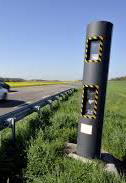
\includegraphics[scale=1]{image/radar.png}\end{center}
\end{multicols}
\begin{enumerate}
    \item Que représentent les variables \mintinline{python3}{h} et \mintinline{python3}{v} ?
    
    \medskip\prof{\mintinline{python3}{h} représente la vitesse et \mintinline{python3}{h} la hauteur des véhicules.}\dotfill
    
    \item Que représentent les valeurs 2 ; 90 et 130 ?
    
    \medskip\prof{la valeur 2 représente la limite de hauteur en mètre  entre VL et VL, 90 et 130 les limites de vitesses.}\dotfill
    
    \item Quelle est le type de la variable << \mintinline{python3}{enFaute} >> ?
    
    \medskip\prof{La variable << \mintinline{python3}{enFaute} est de type Booléen (attention, \mintinline{python3}{type(enFaute)} renvoie une erreur : variable locale à la fonction).}\dotfill
    
    \item Quelles sont les réponses à \mintinline{python3}{Amende(3,100)} et \mintinline{python3}{Amende(1.8,110)} ?
    
    \medskip\prof{Dans les deux cas :  \mintinline{python3}{False}.}\dotfill
    
    \item Expliquer et corriger l'erreur de programmation qui engendre ce << bug >>.
    
    \medskip\prof{Le \mintinline{python3}{else} ne s'applique qu'au second \mintinline{python3}{if}. Un VL en faute fera donc passer la variable \mintinline{python3}{enFaute} à \mintinline{python3}{True} dans le premier }\dotfill
    
    \medskip\prof{puis à \mintinline{python3}{False} dans le second. On peut corriger en remplaçant le second \mintinline{python3}{if} par \mintinline{python3}{elif}.}\dotfill
\end{enumerate}


\subsubsection{Forfait de ski}

Dans la Station de ski de LaRoche, un forfait journée, coûte 35 €. Les enfants de moins de 5 ans ne paient pas pour skier. Ceux de 6 à 17 ans et de plus de 65 ans ont une remise de 20\%.

\begin{enumerate}
    \item Proposer un ensemble de tests qui permettront de vérifier le bon fonctionnement d'un programme qui déterminerait le prix du forfait journée à payer en fonction de l'âge.
    
    \medskip\prof{Il faudrait par exemple tester les âges autour des changements :}\dotfill
    
    \medskip\prof{5 $\Rightarrow$ 0 ; 6 $\Rightarrow$ 28 ; 17 $\Rightarrow$ 28 ; 18 $\Rightarrow$ 35 ; 64 $\Rightarrow$ 35 ; 65 $\Rightarrow$ 28}\dotfill
    
    \item Compléter les programmes suivants, rédigés sous Python, pour déterminer le prix du forfait à payer en fonction de l'âge.
    
    \begin{multicols}{3}
    
\begin{python}[escapeinside=||]
def prix_forfait_1(age):
    if |\prof{age<6 :}|
        prix = 0
    else :
        if |\prof{age<18 or age>64 :}|
            prix = |\prof{28}|
        else :
            prix = 35
    return |\prof{prix}|
\end{python}
\columnbreak
    
\begin{python}[escapeinside=||]
def prix_forfait_1(age):
    if |\prof{age<6 :}|
        prix = 0
    elif |\prof{age>17 and age<65 :}|
        prix = 35
    else :
        prix = |\prof{28}|
    return |\prof{prix}|
\end{python}
\columnbreak
    
\begin{python}[escapeinside=||]
def prix_forfait_3(age):
    prix = |\prof{28}|
    if |\prof{18<=age<=64 :}|
        prix = 35
    if |\prof{age<=5 :}|
        prix = 0
    return |\prof{prix}|
\end{python}
    \end{multicols}
    
    
\end{enumerate} 

\newpage

\subsection{Boucles}

\begin{multicols}{2}

Dans cette partie, on considère le programme ci-dessous, d'une fonction mathématique $f$
dont on donne ci-contre une représentation graphique.

\begin{python}
def f(x):
    y = x*x-1
    if  y < 0 :
        y = -y
    return y
\end{python}

{\centering\def \Xmin {-3.5} \def \Ymin {-0.5} \def \Xmax {3.5} \def \Ymax {3.5}
\begin{tikzpicture}[baseline,line cap=round, line join=round, >=latex, x=1cm, y=1cm, scale=1]
% Grille
\draw [color=black, dotted, xstep=5mm, ystep=5mm] (\Xmin,\Ymin) grid (\Xmax,\Ymax);
\draw[->,color=black] (\Xmin,0) -- (\Xmax,0);
\draw[->,color=black] (0,\Ymin) -- (0.,\Ymax);
\foreach \x in {-1,...,\Xmin,,1,...,\Xmax}
	\draw[shift={(\x,0)},color=black] (0pt,2pt) -- (0pt,-2pt) node[below] {\footnotesize $\x$};
\foreach \y in {1,...,\Ymax}
	\draw[shift={(0,\y)},color=black] (2pt,0pt) -- (-2pt,0pt) node[left] {\footnotesize $\y$};
\draw[shift={(0,0)},color=black] (0pt,-2pt) node[below right] {\footnotesize $0$};
\clip (\Xmin,\Ymin) rectangle (\Xmax,\Ymax);
\draw[thick,smooth,samples=100,domain=-3.5:-1] plot(\x,{\x*\x-1});
\draw[thick,smooth,samples=100,domain=-1:1] plot(\x,{1-\x*\x});
\draw[thick,smooth,samples=100,domain=1:3.5] plot(\x,{\x*\x-1});
\end{tikzpicture}\par}
\end{multicols}

\medskip
\begin{enumerate}
    \item En donner une expression algébrique : $f(x)=$\prof{$\left\lbrace\begin{matrix}1-x^2 & \text{si }x\in[-1;1]\\x^2-1 & \text{sinon}\end{matrix}\right.$ \qquad ou $\vert x^2-1 \vert$}\dotfill
    
    \medskip
    \item Étant donné un nombre réel $a$ compris entre 0 et 8, on cherche à déterminer à \np{0,1} près le plus grand nombre réel $x$ appartement à $[\mintinline{python3}{xmin} ; \mintinline{python3}{xmax}]$ et vérifiant $f(x)\leqslant a$. On propose plusieurs programmes qu'il s'agit de tester et de corriger.
    
    \begin{enumerate}
        \item Premier programme
        
        \begin{multicols}{2}
        Tester le programme ci-contre pour $a=\np{0.5}$, $\mintinline{python3}{xmin}=-1$ et $\mintinline{python3}{xmax}=0$.
        
        \begin{itemize}
            \item Que constate-t-on ? 
            
            \medskip\prof{La valeur renvoyée x=\np{-0.7} donne f(x)>a.}\dotfill
                        
            \item Expliquer l'erreur.
            
            \medskip\prof{La boucle s'arrête quand f(x) n'est plus <=a.}\dotfill
            
             \medskip\prof{On ajoute donc 0,1 de trop.}\dotfill
        \end{itemize}
        
        \columnbreak
        
\begin{python}
def solution1(a, xmin, xmax):
    x = xmin
    while f(x)<=a :
        x = x + 0.1
    return x
\end{python}
        \end{multicols}
        
        
        \item Pour corriger ce programme, on modifie la valeur à renvoyer :
        
        \begin{multicols}{2}
        Donner les valeurs (à \np{0.01} près) renvoyées par :
        
        \begin{itemize}
            \item \mintinline{python3}{solution2(0.5, -1, 0)} \prof{\np{-0.6}}\dotfill
                        
            \item \mintinline{python3}{solution2(0.5, -1, 1)} \prof{\np{-0.6}}\dotfill
                        
            \item \mintinline{python3}{solution2(0.5, -1, 3)} \prof{\np{-0.6}}\dotfill
        \end{itemize}
        
        Expliquer l'erreur de ce programme.
        
        \medskip\prof{Il s'arrête à la première des valeurs ne donnant pas $f(x)\leqslant a$}\dotfill
        
        \medskip\prof{Il devrait s'arrêter à la dernière donnant $f(x)\leqslant a$}\dotfill
        
        \columnbreak
        
\begin{python}
def solution2(a, xmin, xmax):
    x = xmin
    while f(x)<=a :
        x = x + 0.1
    return x - 0.1
\end{python}
        \end{multicols}
        
        \item Compléter le programme ci-dessous pour qu'il réponde au problème initial.
        
\begin{python}[escapeinside=||]
def solution3(a, xmin, xmax):
    x = xmin
    solution = None
    while |\prof{x <= xmax :}|
        if |\prof{f(x)<=a :}|
            solution = |\prof{x}|
        x = x + 0.1
    return solution
\end{python}

\item Que penser du programme suivant ?
        
\begin{python}
def solution4(a, xmin, xmax):
    x = xmax
    while f(x)>a :
        x = x - 0.1
    return x
\end{python}

\medskip\prof{Il répond correctement au tests précédents, mais il vaut mieux éviter de faire une demande avec un $a$ négatif...}\dotfill
        
    \end{enumerate}
    
\end{enumerate}


\chapter{Intelligence artificielle}


L'intelligence artificielle, en tant que domaine de recherche, est née officiellement en 1956, expression proposée par un chercheur américain, John McCarthy. L'article fondateur est celui de Alan Turing en 1950 << Computing machinery and intelligence >>. Il y propose de considérer la question suivante : << Est-ce que les machines peuvent penser ? >>. Il propose un test, dit << jeu de l'imitation >>, passé à la postérité sous le nom de << test de Turing >> : un ordinateur passe le test s'il arrive à se faire passer pour un interlocuteur humain pendant quelques minutes d'un jeu de questions-réponses.


\section{Qu'est-ce que l'intelligence artificielle ?}

Citer, d'après les documents suivants, les grands enjeux de l'intelligence artificiels et la façon dont ils sont traités.

\medskip\prof{Reconnaissance d'images, de textes, de sons, de phrases.}\dotfill

\medskip\prof{Production de réponses adaptées à un interlocuteur ; dans un jeu ; pour conduite une voiture ; faire un diagnostique médical...}\dotfill

\medskip\prof{Longtemps basés sur des règles expertes, le Big Data et les cartes graphiques modernes ont favorisées la programmation d'apprentissages.}\dotfill

\subsubsection{document 1 - Les enjeux de la recherche en intelligence artificielle - Y. Lecun - 2016}


\begin{center}\fbox{\begin{minipage}{0.9\linewidth}Qu'est-ce que l'intelligence ? Est-ce la capacité à percevoir le monde, à prédire le futur immédiat ou lointain, ou à planifier une série d'actions pour atteindre un but ? Est-ce la capacité d'apprendre, ou celle d'appliquer son savoir à bon escient ? La définition est difficile à cerner.

On pourrait dire que l'intelligence artificielle (IA) est un ensemble de techniques permettant à des machines d'accomplir des tâches et de résoudre des problèmes normalement réservés aux humains et à certains animaux.

Les tâches relevant de l'IA sont parfois très simples pour les humains, comme par exemple reconnaître et localiser les objets dans une image, planifier les mouvements d'un robot pour attraper un objet, ou conduire une voiture. Elles requièrent parfois de la planification complexe, comme par exemple pour jouer aux échecs ou au Go. Les tâches les plus compliquées requièrent beaucoup de connaissances et de sens commun, par exemple pour traduire un texte ou conduire un dialogue.

Depuis quelques années, on associe presque toujours l'intelligence aux capacités d'apprentissage. C'est grâce à l'apprentissage qu'un système intelligent capable d'exécuter une tâche peut améliorer ses performances avec l'expérience. C'est grâce à l'apprentissage qu'il pourra apprendre à exécuter de nouvelles tâches et acquérir de nouvelles compétences.

Le domaine de l'IA n'a pas toujours considéré l'apprentissage comme essentiel à l'intelligence. Par le passé, construire un système intelligent consistait à écrire un programme << à la main >> pour jouer aux échecs (par recherche arborescente), reconnaître des caractères imprimés (par comparaison avec des images prototypes), ou faire un diagnostic médical à partir des symptômes (par déduction logique à partir de règles écrites par des experts). Mais cette approche « manuelle » a ses limites.
\end{minipage}}\end{center}

\subsubsection{document 2 - Computing machinery and intelligence - A. Turing - 1950}
\begin{center}\fbox{\begin{minipage}{0.9\linewidth}Au lieu de produire un programme qui simule l'esprit d'un adulte, pourquoi ne pas plutôt essayer d'en produire un qui simule celui de l'enfant ? S'il était alors soumis à une éducation appropriée, on aboutirait au cerveau humain. [...] Nous avons en conséquence divisé le problème en deux parties : le programme-enfant et le processus d'éducation.

[...]

Nous pouvons espérer que les machines concurrenceront finalement l'homme dans tous les champs purement intellectuels. Mais par lesquels vaut-il mieux commencer ? Même cette décision est difficile à prendre. Beaucoup de gens pensent qu'une activité très abstraite comme le jeux d'échec serait la meilleure. On peut aussi soutenir qu'il vaut mieux équiper la machine avec les meilleurs organes sensoriels que l'on puisse acheter, puis lui apprendre à comprendre et à parler anglais. Ce processus pourrait se conformer à l'enseignement normal d'un enfant. On lui montrerait et nommerait des objets, etc.\end{minipage}}\end{center}

\section{Exemple d'intelligence artificielle sur des règles d'experts}

\subsection{L'algorithme MinMax}

Il est basé sur l'évaluation des situations de jeux en terme de score pour le joueur dont c'est le tour. Il suppose que ce joueur cherchera toujours à maximiser ce score alors que son adversaire cherchera à le minimiser.

\medskip

% définition des styles
\tikzstyle{lien}=[->,>=stealth,rounded corners=5pt,thick,baseline]
\tikzset{max/.style={draw=#1,fill=#1!33,text width=0.4cm,align=center},
max/.default={blue}}
\tikzset{min/.style={draw=#1,circle,inner sep=1pt,fill=#1!33,text width=0.5cm,align=center},
min/.default={red}}

\begin{multicols}{2}
{\bfseries Étape 1} : on construit l'arbre des possibles.

\tikz[baseline=(M.base)]\node(M)[max]{$S$}; situation alors que c'est au tour du joueur.

\tikz[baseline=(M.base)]\node(M)[min]{$S$}; situation alors que c'est à son adversaire.

\tikz[baseline=(M.base)]\draw[-latex](0,0)--(0.5,0);  coup joué amenant à une nouvelle situation.

{\centering
\begin{tikzpicture}
[edge from parent path={[->,>=latex](\tikzparentnode) to [out=-90,in=90] (\tikzchildnode)},
level 1/.style={sibling distance=2.25cm,level distance=1cm},
level 2/.style={sibling distance=0.75cm}]
\node [max] {$S_0$}
child{ node [min]{$S_A$}
	child{ node [max]{$S_1$}}
	child{ node [max]{$S_2$}}
	child{ node [max]{$S_3$}}
}
child{ node [min=red]{$S_B$}
	child{ node [max]{$S_4$}}
	child{ node [max]{$S_5$}}
	child{ node [max]{$S_6$}}
}
child{ node [min=red]{$S_C$}
	child{ node [max]{$S_7$}}
	child{ node [max]{$S_8$}}
	child{ node [max]{$S_9$}}
};
\end{tikzpicture}\par}

\medskip

{\bfseries Étape 2} : On évalue le score des situations de jeux du dernier niveau. (Plus il est élevé plus la situation est favorable au joueur.) Imaginons obtenues les évaluations suivantes :

{\centering\begin{tikzpicture}
\foreach \i/\val in {0/7,1/8,2/3,3/2,4/9,5/1,6/6,7/4,8/5}
\node[max,xshift=\i*0.75cm]{$\val$};
\end{tikzpicture}\par}

\columnbreak

{\bfseries Étape 3} : On remonte ces évaluations. 

Comme l'adversaire cherche à minimiser le score du jour, on remonte sur les \tikz[baseline=(M.base)]\node(M)[min]{$S$}; par l'évaluation {\bfseries{}Min}imale des coups possibles.

Comme le joueur cherche à maximiser le score, on remonte sur les \tikz[baseline=(M.base)]\node(M)[max]{$S$}; par l'évaluation {\bfseries{}Max}imale des coups possibles.

{\centering\begin{tikzpicture}
[edge from parent path={[->,>=latex](\tikzparentnode) to [out=-90,in=90] (\tikzchildnode)},
level 1/.style={sibling distance=2.25cm,level distance=1cm},
level 2/.style={sibling distance=0.75cm}]
\node(C)[max] {$\mathbf{4}$}
child{ node(G)[min]{$3$}
	child{ node [max]{$7$}}
	child{ node [max]{$8$}}
	child{ node(F)[max]{$3$}}
}
child{ node(E)[min=red]{$1$}
	child{ node [max]{$2$}}
	child{ node [max]{$9$}}
	child{ node(D)[max]{$1$}}
}
child{ node(B)[min=red]{$\mathbf{4}$}
	child{ node [max]{$6$}}
	child{ node(A)[max]{$\mathbf{4}$}}
	child{ node [max]{$5$}}
};

\draw[line width=1pt,-latex] (A)to [out=0,in=-45](B);
\node[right=0.75cm] at ($0.5*(A)+0.5*(B)$){\bfseries Min};
\draw[line width=1pt,-latex] (B)to [out=180,in=0](C);
\node[right] at ($0.5*(B)+0.5*(C)$){\bfseries Max};
\draw[line width=1pt,-latex] (D)to [out=180,in=-45](E);
\draw[line width=1pt,-latex] (F)to [out=180,in=-45](G);
\end{tikzpicture}\par}


On en déduit le meilleur coup à jouer. 

Ici c'est le troisième : C.

\end{multicols}

Les étapes 1 et 3 sont les mêmes, quelque soit le jeu choisi. L'étape 2 est plus délicate, car l'évaluation du score peut être subjectif. Par exemple : combien vaut un pion comparé à une dame aux échecs ? On a donc, besoin de l'avis d'un expert.

\subsection{Application au morpion}

Après consultation d'un expert, on met en place la fonction de score suivante :

\begin{itemize}
    \item 3 marques identiques alignées valent 1000 points.
    \item 2 marques identiques alignées avec un case libre valent 100 points.
    \item 1 marque alignée avec 2 cases libres valent 10 points.
    \item Les autres alignements valent 0 point.
    \item Ces points sont comptés positivement si ce sont les marques du joueur, négativement sinon.
\end{itemize}

Exemple d'une évluation d'une situation de jeu pour le joueur \tikz[scale=0.3]\draw[red](0,0)--(1,1)(0,1)--(1,0); : 

{\centering
 \begin{tikzpicture}[scale=0.3,baseline=(A).base]\coordinate(A)at(0.5,0.5);
\foreach \i in {0,1,2,3} \draw(0,\i)--(3,\i)(\i,0)--(\i,3);
\draw[red](0,2)--(1,3)(0,3)--(1,2);
\draw[blue](1.5,1.5)circle(0.4);
\draw[line width=2pt,red](0,0)rectangle(1,3);
\node at(1.5,-1){$+10$};
\end{tikzpicture}
\begin{tikzpicture}[scale=0.3,baseline=(A).base]\coordinate(A)at(0.5,0.5);
\foreach \i in {0,1,2,3} \draw(0,\i)--(3,\i)(\i,0)--(\i,3);
\draw[red](0,2)--(1,3)(0,3)--(1,2);
\draw[blue](1.5,1.5)circle(0.4);
\draw[line width=2pt,blue](2,0)rectangle(1,3);
\node at(1.5,-1){$-10$};
\end{tikzpicture}
\begin{tikzpicture}[scale=0.3,baseline=(A).base]\coordinate(A)at(0.5,0.5);
\foreach \i in {0,1,2,3} \draw(0,\i)--(3,\i)(\i,0)--(\i,3);
\draw[red](0,2)--(1,3)(0,3)--(1,2);
\draw[blue](1.5,1.5)circle(0.4);
\draw[line width=2pt,blue](3,0)rectangle(2,3);
\node at(1.5,-1){$+0$};
\end{tikzpicture}
\begin{tikzpicture}[scale=0.3,baseline=(A).base]\coordinate(A)at(0.5,0.5);
\foreach \i in {0,1,2,3} \draw(0,\i)--(3,\i)(\i,0)--(\i,3);
\draw[red](0,2)--(1,3)(0,3)--(1,2);
\draw[blue](1.5,1.5)circle(0.4);
\draw[line width=2pt,red](3,2)rectangle(0,3);
\node at(1.5,-1){$+10$};
\end{tikzpicture}
\begin{tikzpicture}[scale=0.3,baseline=(A).base]\coordinate(A)at(0.5,0.5);
\foreach \i in {0,1,2,3} \draw(0,\i)--(3,\i)(\i,0)--(\i,3);
\draw[red](0,2)--(1,3)(0,3)--(1,2);
\draw[blue](1.5,1.5)circle(0.4);
\draw[line width=2pt,blue](3,1)rectangle(0,2);
\node at(1.5,-1){$-10$};
\end{tikzpicture}
\begin{tikzpicture}[scale=0.3,baseline=(A).base]\coordinate(A)at(0.5,0.5);
\foreach \i in {0,1,2,3} \draw(0,\i)--(3,\i)(\i,0)--(\i,3);
\draw[red](0,2)--(1,3)(0,3)--(1,2);
\draw[blue](1.5,1.5)circle(0.4);
\draw[line width=2pt,blue](3,1)rectangle(0,0);
\node at(1.5,-1){$+0$};
\end{tikzpicture}
\begin{tikzpicture}[scale=0.3,baseline=(A).base]\coordinate(A)at(0.5,0.5);
\foreach \i in {0,1,2,3} \draw(0,\i)--(3,\i)(\i,0)--(\i,3);
\draw[red](0,2)--(1,3)(0,3)--(1,2);
\draw[blue](1.5,1.5)circle(0.4);
\draw[line width=2pt,blue,rotate=45](0,-0.5)rectangle(4.24,0.5);
\node at(1.5,-1){$-10$};
\end{tikzpicture}
\begin{tikzpicture}[scale=0.3,baseline=(A).base]\coordinate(A)at(0.5,0.5);
\foreach \i in {0,1,2,3} \draw(0,\i)--(3,\i)(\i,0)--(\i,3);
\draw[red](0,2)--(1,3)(0,3)--(1,2);
\draw[blue](1.5,1.5)circle(0.4);
\draw[line width=2pt,blue,rotate=-45,xshift=-2.1cm,yshift=2.1cm](0,-0.5)rectangle(4.24,0.5);
\node at(1.5,-1){$+0$};
\end{tikzpicture}
\begin{tikzpicture}[scale=0.3,baseline=(A).base]\coordinate(A)at(0.5,0.5);
\foreach \i in {0,1,2,3} \draw(0,\i)--(3,\i)(\i,0)--(\i,3);
\draw[red](0,2)--(1,3)(0,3)--(1,2);
\draw[blue](1.5,1.5)circle(0.4);
\node at(1.5,-1){$=-10$};
\end{tikzpicture}
\par}

On se propose de déterminer ce que serait le premier coup du MinMax avec cette évaluation dans une grille vide. Compléter (en ne considérant pas les situations symétriques) :

{\centering
\begin{tikzpicture}[scale=0.35]
\foreach \k in {0,...,11} 
    \foreach \i in {0,1,2,3} \draw[xshift={\k*3.5cm}](0,\i)--(3,\i)(\i,0)--(\i,3);
\foreach \k in {0,1,7,8,9,10,11}
    \draw[xshift={\k*3.5cm}](1.5,-1.5)node{\pointsuite{1cm}};
\foreach \k/\val in {2/10, 3/0, 4/-10, 5/10, 6/0}
    \draw[xshift={\k*3.5cm}](1.5,-1)node{$\val$};
\foreach \i in {0,1,2,3} \draw[xshift={1.75cm},yshift={5cm}](0,\i)--(3,\i)(\i,0)--(\i,3);
    \draw[red,xshift={1.75cm},yshift={5cm}](1,1)--(2,2)(1,2)--(2,1);
    \draw[xshift={1.75cm},yshift={5cm}](3,1.5)node[right]{Min = \pointsuite{1cm}};
\foreach \i in {0,1,2,3} \draw[xshift={4*3.5cm},yshift={5cm}](0,\i)--(3,\i)(\i,0)--(\i,3);
    \draw[red,xshift={4*3.5cm},yshift={5cm}](0,2)--(1,3)(0,3)--(1,2);
    \draw[xshift={4*3.5cm},yshift={5cm}](3,1.5)node[right]{Min = $-10$};
\foreach \i in {0,1,2,3} \draw[xshift={9*3.5cm},yshift={5cm}](0,\i)--(3,\i)(\i,0)--(\i,3);
    \draw[red,xshift={9*3.5cm},yshift={5cm}](1,2)--(2,3)(1,3)--(2,2);
    \draw[xshift={9*3.5cm},yshift={5cm}](3,1.5)node[right]{Min = \pointsuite{1cm}};
\foreach \i in {0,1,2,3} \draw[xshift={5*3.5cm+1.75cm},yshift={10cm}](0,\i)--(3,\i)(\i,0)--(\i,3);
    \draw[xshift={5*3.5cm+1.75cm},yshift={10cm}](3,1.5)node[right]{Max = \pointsuite{1cm}};
\foreach \k in {0,1} \draw[-latex]({3.25},5)to [out=-90,in=90]({\k*3.5+1.75},3);
\foreach \k in {2,...,6} {
    \draw[-latex]({4*3.5+1.5},5)to [out=-90,in=90]({\k*3.5+1.75},3);
    \draw[red,xshift={\k*3.5cm}](0,2)--(1,3)(0,3)--(1,2);
}
    \draw[blue,xshift={2*3.5cm}](1.5,2.5)circle(0.4);
    \draw[blue,xshift={3*3.5cm}](2.5,2.5)circle(0.4);
    \draw[blue,xshift={4*3.5cm}](1.5,1.5)circle(0.4);
    \draw[blue,xshift={5*3.5cm}](2.5,1.5)circle(0.4);
    \draw[blue,xshift={6*3.5cm}](2.5,0.5)circle(0.4);
\foreach \k in {7,...,11} \draw[-latex]({9*3.5+1.5},5)to [out=-90,in=90]({\k*3.5+1.75},3);
\draw[-latex]({6*3.5-0.25},10)to [out=-20,in=130]({9*3.5+1.5},8);
\draw[-latex]({6*3.5-0.25},10)to [out=-90,in=90]({4*3.5+1.5},8);
\draw[-latex]({6*3.5-0.25},10)to [out=-160,in=50]({3.25},8);
\end{tikzpicture}
\par}

\section{L'apprentissage machine}

Aussi connu sous le nom d'apprentissage artificiel ou d'apprentissage automatique, il
consiste en des programmes capables d'ajuster leur comportement à des données dites
d'entraînement. On distingue communément trois modalités principales d'apprentissage.

\begin{itemize}
    \item L'apprentissage {\bfseries supervisé}, consiste à apprendre à une machine à catégoriser des données à partir d'un grand nombre de données préalablement étiquetées par l'Homme. Pendant la phase d'apprentissage, on calibre un algorithme en adaptant ses paramètres de catégorisation aux données fournies. On utilise ensuite cet algorithme pour catégoriser de nouvelles données.
    \item L'apprentissage {\bfseries non supervisé}, consiste à fournir à la machine un grand nombre données, non étiquetées. La machine y repère des régularités, des proximités, des corrélations pour construire elle-même son algorithme de classification.
    \item L'apprentissage {\bfseries par renforcement} consiste à induire le comportement d'un << agent >> (par exemple un robot) évoluant dans un << environnement >> (par exemple dans une pièce où il doit manipuler des objets) et qui apprend grâce à un système de << récompenses >>.
\end{itemize} 

\medskip
Les exemples développés ici sont issues de l'apprentissage supervisé.

\subsection{Ajustement linéaire}

En mathématiques, un ajustement linéaire est la détermination d'une droite approchant au mieux un nuage de points dans le plan.

%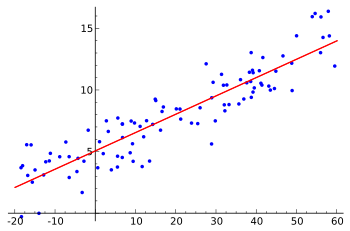
\includegraphics[scale=1]{image/Linear_regression.svg}

\subsubsection{Méthode de Mayer}

Dans le cas où les abscisses sont différentes deux à deux, elles peuvent être ordonnées et la Méthode de Mayer (parmi d'autres) consiste à partager le nuage de points en deux de tailles égales selon la valeur de leurs abscisses (les petite d'une part, les grandes d'autre part). La droite retenue est alors celle qui passe par le point moyen de chacun des deux nuages.

\begin{enumerate}
    \item Justifier qu'il s'agit d'un algorithme d'apprentissage supervisé.
    
    \medskip  Les données fournies sont \prof{les abscisses avec comme << catégories >> les ordonnées des points du nuage.}\dotfill
    
    \medskip Adapter les paramètres, c'est \prof{déterminer le coefficient directeur et l'ordonnée à l'origine de la droite.}\dotfill
    
    \medskip Catégoriser de nouvelles données, c'est \prof{associée à chaque autre abscisse l'ordonnée correspondante sur la droite.}\dotfill
    \item Appliquer cette méthode dans le contexte suivant : prix du m$^2$ dans le 6$^e$ arrondissement de Paris.
    
    \begin{tabular}{ccccccccccccccccccccc}
    Année $200x_i$ & 0 & 1 & 2 & 3 & 4 & 5 & 6 & 7 & 8 & 9 \\
    Prix au m$^2$ $y_i$ & 4562 & 5270 & 5400 & 6020 & 6460 & 7360 & 8090 & 8840 & 9830 & 10100 \\
    \multicolumn{11}{c}{\footnotesize}\\
    Année $200x_i$ & 10 & 11 & 12 & 13 & 14 & 15 & 16 & 17 & 18 & 19\\
    Prix au m$^2$ $y_i$ & 9690 & 11870 & 12400 & 12250 & 11820 & 11280 & 12150 & 12320 & 12530 & 13880 \\
    \end{tabular}
    
    \medskip Points moyens : \prof{$(\np{2004,5} ; \np{7193,2})$ et $(\np{2014,5} ; 12019)$}\dotfill
    
    Tracer la droite correspondante sur la représentation ci-dessous :
    
{\centering\def \Xmin {0} \def \Ymin {0} \def \Xmax {20} \def \Ymax {16}
\begin{tikzpicture}[baseline,line cap=round, line join=round, >=latex, x=0.5cm, y=0.25cm, scale=1]
% Grille
\draw [color=black, dotted, xstep=5mm, ystep=5mm] (\Xmin,\Ymin) grid (\Xmax,\Ymax);
\draw[->,color=black] (\Xmin,0) -- (\Xmax,0);
\draw[->,color=black] (0,\Ymin) -- (0.,\Ymax);
\foreach \x in {0,1,...,\Xmax}
	\draw[shift={(\x,0)},color=black] (0pt,2pt) -- (0pt,-2pt) node[below] {\footnotesize $\x$};
\foreach \y in {0,2,...,\Ymax}
	\draw[shift={(0,\y)},color=black] (2pt,0pt) -- (-2pt,0pt) node[left] {\footnotesize $
\y$\ifnum\y>0{000}\fi};

\setcounter{x}{0}
\foreach \y in {4562,5270,5400,6020,6460,7360,8090,8840,9830,10100,9690,11870,12400,12250,11820,11280,12150 ,12320,12530,13880} {\node[]at(\thex,{\y/1000}){$\bullet$}; \stepcounter{x}}

\draw (0,4.562)
\foreach \x/\y in {0/4562, 1/5270, 2/5400, 3/6020, 4/6440, 5/7360, 6/8090, 7/8840, 8/9830, 9/10100, 10/9690, 11/11870, 12/12400, 13/12250, 14/11820, 15/11280, 16/12150, 17/12320, 18/12530, 19/13880} { -- (\x,{\y/1000})};

%\draw[thick,smooth,dashed,blue,samples=100,domain=\Xmin:\Xmax] plot(\x,{0.47349*\x + 5.1079});
%\draw[thick,smooth,dashed,samples=100,domain=\Xmin:\Xmax] plot(\x,{((7.1932-12.019)/(4.5-14.5))*(\x - 4.5) + 7.1932});
%\node[]at(4.5,7.1932){$\times$};
%\node[]at(14.5,12.019){$\times$};
%\node[]at(9.5,9.6061){\color{red}$\times$};
\end{tikzpicture}\par}
\end{enumerate}

\subsubsection{Méthode des moindres carrés}

C'est une méthode statistique permettant de trouver la << meilleure >> droite, selon certains critères. Dans l'exemple précédent, elle donne : $y = \np{473,49} x + \np{5107,9}$. 

\medskip À quel prix au m$^2$ peut-on s'attendre pour 2020 ? \prof{$\np{473,49} \times 20 + \np{5107,9} \approx 14578$}\dotfill


\subsection{Le Perceptron}

\subsubsection{La machine}

L'invention du perception suit l'idée de A. Turing de construire un jeune cerveau que l'on puisse instruire. De manière plus élémentaire, il s'agit de modéliser un neurone du cerveau avec ses synapses. 


{\centering\includegraphics[height=4cm]{image/Perceptron1.jpg}
\includegraphics[height=4cm]{image/Perceptron2.jpg}
\includegraphics[height=4cm]{image/Perceptron3.png}\par}


La machine est constituée d'une rétine pour de percevoir une image simple (à gauche ; très basse résolution : quelques pixels), d'une aire associative permet de fournir les valeurs d'entrée (au milieu ; les synapses) le tout relié à un classifieur (le neurone) qui fait la somme de ces valeurs après les avoir multipliées par des poids (donnés par des potentiomètres motorisés ; à droite) et donnant en sortie la classe de l'image perçu par une fonction en escalier.


{\centering\begin{tikzpicture}[scale=0.3]
\node[]at(3,0.5){\scriptsize Rétine};
\draw(0,-1)--(6,0)--(6,-7)--(0,-8)--cycle;
\node[]at(10,0.5){\scriptsize Valeurs};
\node[](V1)at(10.5,-1){$x_1$};
\node[]at(10.5,-2.3){$\vdots$};
\node[](V2)at(10.5,-4){$x_i$};
\node[]at(10.5,-5.3){$\vdots$};
\node[](V3)at(10.5,-7){$x_n$};
\draw(V1.west)--++(-3,-0.75);
\draw(V1.west)--++(-3,0.75);
\draw(V3.west)--++(-3,-0.75);
\draw(V3.west)--++(-3,0.75);
\node[text width=1.5cm,left, align=center]at(V2.west){\scriptsize Aire\\associative};
\node[]at(14.5,-0.5){\scriptsize Poids};
\node[text width=0.75cm,minimum size=0.75cm,circle,inner sep=0, draw,align=center](S)at(19,-4){$\Sigma$};
\draw[-latex](V1)--(S)node[midway,text width=0.4cm,minimum size=0.4cm,inner sep=0, draw,align=center,fill=white]{$p_1$};
\draw[-latex](V2)--(S)node[midway,text width=0.4cm,minimum size=0.4cm,inner sep=0, draw,align=center,fill=white]{$p_i$};
\draw[-latex](V3)--(S)node[midway,text width=0.4cm,minimum size=0.4cm,inner sep=0, draw,align=center,fill=white]{$p_n$};
\node[text width=0.75cm,minimum size=0.75cm,circle,inner sep=0, draw,align=center](E)at(23,-4){\tikz\draw(0,0)--(0.1,0)--(0.1,0.2)--(0.2,0.2);};
\node[inner sep = 2pt](O)at(27,-4){};
\draw[-latex](S)--(E)node[midway,above=0.5cm]{\scriptsize Classifieur};
\draw[-latex](E)--(O)node[right]{\scriptsize $\displaystyle \text{sign}\left(\sum_{i=1}^n p_i x_i + b\right)$};
\end{tikzpicture}\par}


L'apprentissage consiste alors en la modification automatique des poids selon la réponse.


\subsubsection{Un exemple : distinguer un << A >> d'un << B >>}

On ne considère que 3 synapses pour simplifier. Voyons comment le Perceptron apprend à reconnaitre un << A >> d'un << B >>. L'entrée << A >> doit renvoyer une sortie positive et l'entrée  << B >> une sortie négative.

\begin{multicols}{2}
On choisit un réglage de départ neutre : chaque poids à 0. O présente l'image d'un << A >>, pour laquelle on associe blanc à 0 et noir à 1, avec l'indication de la sortie attendue : 1. On obtient le schéma ci-contre. 
    
\begin{center}\begin{tikzpicture}[scale=0.3]
\setcounter{x}{0}\setcounter{y}{0}
\foreach \k in {
  0,0,0,0,0,0,0,0,
  0,0,0,1,0,0,0,0,
  0,0,0,1,1,0,0,0,
  0,0,1,0,0,1,0,0,
  0,0,1,1,1,1,0,0,
  0,1,0,0,0,0,1,0,
  0,1,0,0,0,0,1,0,
  0,0,0,0,0,0,0,0} {
    \ifnum\k=1{\fill(\thex cm,-\they cm)rectangle++(1,-1);}\fi
    \stepcounter{x}
    \ifnum\thex=8{\stepcounter{y}\setcounter{x}{0}}\fi
}
\draw [thick, black!50, step=1.0cm] (0,-8) grid (8,0);
%\node[]at(10,0.5){Valeurs};
\node[inner sep = 0](P1)at(1.5,-1.5){\color{red}$\bullet$};
\node[inner sep = 0](P2)at(3.5,-2.5){\color{red}$\bullet$};
\node[inner sep = 0](P3)at(3.5,-6.5){\color{red}$\bullet$};
\node[](V1)at(10.5,-1){0};
\node[](V2)at(10.5,-4){1};
\node[](V3)at(10.5,-7){0};
\draw[red,-latex](P1)--(V1);
\draw[red,-latex](P2)--(V2);
\draw[red,-latex](P3)--(V3);
%\node[]at(14,0.5){Poids};
\node[text width=0.75cm,minimum size=0.75cm,circle,inner sep=0, draw,align=center](S)at(17,-4){$\Sigma$};
\draw[-latex](V1)--(S)node[midway,text width=0.4cm,minimum size=0.4cm,inner sep=0, draw,align=center,fill=white]{0};
\draw[-latex](V2)--(S)node[midway,text width=0.4cm,minimum size=0.4cm,inner sep=0, draw,align=center,fill=white]{0};
\draw[-latex](V3)--(S)node[midway,text width=0.4cm,minimum size=0.4cm,inner sep=0, draw,align=center,fill=white]{0};
\node[text width=0.75cm,minimum size=0.75cm,circle,inner sep=0, draw,align=center](E)at(21,-4){\tikz\draw(0,0)--(0.1,0)--(0.1,0.2)--(0.2,0.2);};
\draw[-latex](S)--(E)node[midway, above]{0};
\node[inner sep = 2pt](O)at(24,-4){0};
\draw[-latex](E)--(O);
\node[left]at(25,-7){Attendu : 1};
\end{tikzpicture}\end{center}
\end{multicols}
\begin{multicols}{2}
\begin{enumerate}
    \item Comme la sortie est inférieure à l'attendu, le Perceptron augmente chacun des poids correspondants à une case noire d'une unité. Reporter les nouveaux poids sur le schéma ci-contre et compléter par rapport à la situation.
\end{enumerate}
    
\begin{center}\begin{tikzpicture}[scale=0.3]
\setcounter{x}{0}\setcounter{y}{0}
\foreach \k in {
  0,0,0,0,0,0,0,0,
  0,1,1,1,1,1,0,0,
  0,1,0,0,0,0,1,0,
  0,1,0,0,0,0,1,0,
  0,1,1,1,1,1,0,0,
  0,1,0,0,0,0,1,0,
  0,1,1,1,1,1,0,0,
  0,0,0,0,0,0,0,0} {
    \ifnum\k=1{\fill(\thex cm,-\they cm)rectangle++(1,-1);}\fi
    \stepcounter{x}
    \ifnum\thex=8{\stepcounter{y}\setcounter{x}{0}}\fi
}
\draw [thick, black!50, step=1.0cm] (0,-8) grid (8,0);
%\node[]at(10,0.5){Valeurs};
\node[inner sep = 0](P1)at(1.5,-1.5){\color{red}$\bullet$};
\node[inner sep = 0](P2)at(3.5,-2.5){\color{red}$\bullet$};
\node[inner sep = 0](P3)at(3.5,-6.5){\color{red}$\bullet$};
\node[](V1)at(10.5,-1){\ldots};
\node[](V2)at(10.5,-4){\ldots};
\node[](V3)at(10.5,-7){\ldots};
\draw[red,-latex](P1)--(V1);
\draw[red,-latex](P2)--(V2);
\draw[red,-latex](P3)--(V3);
%\node[]at(14,0.5){Poids};
\node[text width=0.75cm,minimum size=0.75cm,circle,inner sep=0, draw,align=center](S)at(17,-4){$\Sigma$};
\draw[-latex](V1)--(S)node[midway,text width=0.4cm,minimum size=0.4cm,inner sep=0, draw,align=center,fill=white]{\ldots};
\draw[-latex](V2)--(S)node[midway,text width=0.4cm,minimum size=0.4cm,inner sep=0, draw,align=center,fill=white]{\ldots};
\draw[-latex](V3)--(S)node[midway,text width=0.4cm,minimum size=0.4cm,inner sep=0, draw,align=center,fill=white]{\ldots};
\node[text width=0.75cm,minimum size=0.75cm,circle,inner sep=0, draw,align=center](E)at(21,-4){\tikz\draw(0,0)--(0.1,0)--(0.1,0.2)--(0.2,0.2);};
\draw[-latex](S)--(E)node[midway, above]{\ldots};
\node[inner sep = 2pt](O)at(24,-4){\ldots};
\draw[-latex](E)--(O);
\node[left]at(25,-7){Attendu : -1};
\end{tikzpicture}\end{center}
\end{multicols}

\begin{enumerate}\stepcounter{enumi}
    \item Comme la sortie est supérieure à l'attendu, le Perceptron diminue chacun des poids correspondants à une case noire d'une unité. Reporter les nouveaux poids sur les schémas ci-dessous et vérifier que les deux tests sont bien validés.
\end{enumerate}

\begin{multicols}{2}
\begin{center}\begin{tikzpicture}[scale=0.3]
\setcounter{x}{0}\setcounter{y}{0}
\foreach \k in {
  0,0,0,0,0,0,0,0,
  0,0,0,1,0,0,0,0,
  0,0,0,1,1,0,0,0,
  0,0,1,0,0,1,0,0,
  0,0,1,1,1,1,0,0,
  0,1,0,0,0,0,1,0,
  0,1,0,0,0,0,1,0,
  0,0,0,0,0,0,0,0} {
    \ifnum\k=1{\fill(\thex cm,-\they cm)rectangle++(1,-1);}\fi
    \stepcounter{x}
    \ifnum\thex=8{\stepcounter{y}\setcounter{x}{0}}\fi
}
\draw [thick, black!50, step=1.0cm] (0,-8) grid (8,0);
%\node[]at(10,0.5){Valeurs};
\node[inner sep = 0](P1)at(1.5,-1.5){\color{red}$\bullet$};
\node[inner sep = 0](P2)at(3.5,-2.5){\color{red}$\bullet$};
\node[inner sep = 0](P3)at(3.5,-6.5){\color{red}$\bullet$};
\node[](V1)at(10.5,-1){\ldots};
\node[](V2)at(10.5,-4){\ldots};
\node[](V3)at(10.5,-7){\ldots};
\draw[red,-latex](P1)--(V1);
\draw[red,-latex](P2)--(V2);
\draw[red,-latex](P3)--(V3);
%\node[]at(14,0.5){Poids};
\node[text width=0.75cm,minimum size=0.75cm,circle,inner sep=0, draw,align=center](S)at(17,-4){$\Sigma$};
\draw[-latex](V1)--(S)node[midway,text width=0.4cm,minimum size=0.4cm,inner sep=0, draw,align=center,fill=white]{\ldots};
\draw[-latex](V2)--(S)node[midway,text width=0.4cm,minimum size=0.4cm,inner sep=0, draw,align=center,fill=white]{\ldots};
\draw[-latex](V3)--(S)node[midway,text width=0.4cm,minimum size=0.4cm,inner sep=0, draw,align=center,fill=white]{\ldots};
\node[text width=0.75cm,minimum size=0.75cm,circle,inner sep=0, draw,align=center](E)at(21,-4){\tikz\draw(0,0)--(0.1,0)--(0.1,0.2)--(0.2,0.2);};
\draw[-latex](S)--(E)node[midway, above]{\ldots};
\node[inner sep = 2pt](O)at(24,-4){\ldots};
\draw[-latex](E)--(O);
\node[left]at(25,-7){Attendu : 1};
\end{tikzpicture}

\begin{tikzpicture}[scale=0.3]
\setcounter{x}{0}\setcounter{y}{0}
\foreach \k in {
  0,0,0,0,0,0,0,0,
  0,1,1,1,1,1,0,0,
  0,1,0,0,0,0,1,0,
  0,1,0,0,0,0,1,0,
  0,1,1,1,1,1,0,0,
  0,1,0,0,0,0,1,0,
  0,1,1,1,1,1,0,0,
  0,0,0,0,0,0,0,0} {
    \ifnum\k=1{\fill(\thex cm,-\they cm)rectangle++(1,-1);}\fi
    \stepcounter{x}
    \ifnum\thex=8{\stepcounter{y}\setcounter{x}{0}}\fi
}
\draw [thick, black!50, step=1.0cm] (0,-8) grid (8,0);
%\node[]at(10,0.5){Valeurs};
\node[inner sep = 0](P1)at(1.5,-1.5){\color{red}$\bullet$};
\node[inner sep = 0](P2)at(3.5,-2.5){\color{red}$\bullet$};
\node[inner sep = 0](P3)at(3.5,-6.5){\color{red}$\bullet$};
\node[](V1)at(10.5,-1){\ldots};
\node[](V2)at(10.5,-4){\ldots};
\node[](V3)at(10.5,-7){\ldots};
\draw[red,-latex](P1)--(V1);
\draw[red,-latex](P2)--(V2);
\draw[red,-latex](P3)--(V3);
%\node[]at(14,0.5){Poids};
\node[text width=0.75cm,minimum size=0.75cm,circle,inner sep=0, draw,align=center](S)at(17,-4){$\Sigma$};
\draw[-latex](V1)--(S)node[midway,text width=0.4cm,minimum size=0.4cm,inner sep=0, draw,align=center,fill=white]{\ldots};
\draw[-latex](V2)--(S)node[midway,text width=0.4cm,minimum size=0.4cm,inner sep=0, draw,align=center,fill=white]{\ldots};
\draw[-latex](V3)--(S)node[midway,text width=0.4cm,minimum size=0.4cm,inner sep=0, draw,align=center,fill=white]{\ldots};
\node[text width=0.75cm,minimum size=0.75cm,circle,inner sep=0, draw,align=center](E)at(21,-4){\tikz\draw(0,0)--(0.1,0)--(0.1,0.2)--(0.2,0.2);};
\draw[-latex](S)--(E)node[midway, above]{\ldots};
\node[inner sep = 2pt](O)at(24,-4){\ldots};
\draw[-latex](E)--(O);
\node[left]at(25,-7){Attendu : -1};
\end{tikzpicture}\end{center}
\end{multicols}
Source de l'activité : Yann Lecun - Lecture inaugurale au Collège de France en 2016.

\href{https://www.college-de-france.fr/site/yann-lecun/inaugural-lecture-2016-02-04-18h00.htm}{https://www.college-de-france.fr/site/yann-lecun/inaugural-lecture-2016-02-04-18h00.htm}

\section{L'inférence bayésienne}

L'inférence bayésienne fait référence au révérend Thomas Bayes, mathématicien et pasteur
britannique né à Londres aux environs de l'année 1702 et mort en 1761. Ses découvertes en
probabilités ont été résumées dans son << Essai sur la manière de résoudre un problème dans la théorie des risques >> publié à titre posthume en 1763. On lui doit notamment le théorème de Bayes, très utilisé dans tout ce qui relève du classement automatique (diagnostic médical, filtrage de spams).

\subsection{Diagnostique médical}

Une personne vient de passer un test de dépistage d'une maladie rare. On sait qu'elle ne
touche que \np{0,1} \% de la population. Le médecin lui annonce que le résultat du test est positif. La personne demande alors au médecin si le test est fiable. Sa réponse est sans appel : << Si vous êtes malade, le test est positif dans 90 \% des cas et si vous n'êtes pas malade, il est négatif dans 97 \% des cas. >>

Problème posé : {\bfseries quelle est la probabilité que cette personne soit effectivement malade ?}

\begin{multicols}{2}

\begin{enumerate}
    \item Compléter la représentation par un tableau :

(pour \np{10000} personnes.)
\end{enumerate} 

\begin{center}\begin{tabular}{|c|c|c|c|}
\cline{2-4}
\multicolumn{1}{r|}{Test $\rightarrow$} & positif& négatif&  \\
\multicolumn{1}{c|}{Malade $\downarrow$} & $T$ & $\overline{T}$ & Total \\
 \hline
\raisebox{-1.5ex}{\rule{0pt}{2em}}oui : $M$& \prof{\np{9}}\pointsuite{1cm} & \prof{\np{1}}\pointsuite{1cm}  & \prof{\np{10}}\pointsuite{1cm} \\
 \hline
\raisebox{-1.5ex}{\rule{0pt}{2em}}non : $\overline{M}$& \prof{\np{300}}\pointsuite{1cm} & \prof{\np{9690}}\pointsuite{1cm} & \prof{\np{9990}}\pointsuite{1cm}\\
 \hline
\raisebox{-1.5ex}{\rule{0pt}{2em}}Total & \prof{\np{309}}\pointsuite{1cm} & \prof{\np{9691}}\pointsuite{1cm} &  \np{10000} \\
 \hline
\end{tabular}\end{center}

\vfill
~
\
\columnbreak


\begin{enumerate}\stepcounter{enumi}
    \item Compléter la représentation par un arbre :

(probabilités en pourcentages.)
\end{enumerate}


{\centering
\begin{tikzpicture}
\node[text width = 1cm, inner sep = 0pt,align = center,left=0pt](R){$\Omega$\\ \np{10000}};
\node[text width = 1cm, inner sep = 0pt,align = center,right=0pt](M)at($(R.east)+(1.5cm,1cm)$){$M$\\\prof{\np{10}}\pointsuite{1cm}};
\node[text width = 1cm, inner sep = 0pt,align = center,right=0pt](Mn)at($(R.east)+(1.5cm,-1cm)$){$\overline{M}$\\\prof{\np{9990}}\pointsuite{1cm}};
\draw(R.east)--(M.west)node[midway,above]{\np{0.1}\%};
\draw(R.east)--(Mn.west)node[midway,below]{\prof{\np{99.9}\%}\pointsuite{1cm}};
\node[text width = 1cm, inner sep = 0pt,align = center,right=0pt](MT)at($(M.east)+(1.5cm,0.5cm)$){$T$\\\prof{\np{9}}\pointsuite{1cm}};
\node[text width = 1cm, inner sep = 0pt,align = center,right=0pt](MTn)at($(M.east)+(1.5cm,-0.5cm)$){$\overline{T}$\\\prof{\np{1}}\pointsuite{1cm}};
\node[text width = 1cm, inner sep = 0pt,align = center,right=0pt](MnT)at($(Mn.east)+(1.5cm,0.5cm)$){$T$\\\prof{\np{300}}\pointsuite{1cm}};
\node[text width = 1cm, inner sep = 0pt,align = center,right=0pt](MnTn)at($(Mn.east)+(1.5cm,-0.5cm)$){$\overline{T}$\\\prof{\np{9690}}\pointsuite{1cm}};
\draw(M.east)--(MT.west)node[midway,above]{\prof{\np{90}\%}\pointsuite{1cm}};
\draw(M.east)--(MTn.west)node[midway,below]{\prof{\np{10}\%}\pointsuite{1cm}};
\draw(Mn.east)--(MnT.west)node[midway,above]{\prof{\np{3}\%}\pointsuite{1cm}};
\draw(Mn.east)--(MnTn.west)node[midway,below]{\prof{\np{97}\%}\pointsuite{1cm}};
\end{tikzpicture}
\par}
\end{multicols}

On constate que l'arbre donne une importance prépondérante au fait d'être malade ou non par rapport au fait d'avoir un test positif ou négatif, alors que le tableau semble plus symétrique.

\begin{multicols}{2}
\begin{enumerate}\stepcounter{enumi}\stepcounter{enumi}
    \item À l'aide des données du tableau, compléter l'arbre inversé ci-contre en arrondissant les probabilités à $10^{-4}$ près.
    
    \item Quelle est la probabilité qu'une personne positive au test soit effectivement malade ?
    
    \medskip\prof{environ 3\%}\dotfill
    
    \item Pourquoi est-ce contre-intuitif ?
    
    \medskip\prof{Comme un test est positif pour 90 \% des malades et négatif pour}\dotfill
    
    \medskip\prof{97\% des malades, cela laissait penser qu'il était efficace...}\dotfill
\end{enumerate}

\columnbreak
{\centering
\begin{tikzpicture}
\node[text width = 1cm, inner sep = 0pt,align = center,left=0pt](R){$\Omega$\\ \np{10000}};
\node[text width = 1cm, inner sep = 0pt,align = center,right=0pt](M)at($(R.east)+(1.5cm,1cm)$){$T$\\\prof{\np{309}}\pointsuite{1cm}};
\node[text width = 1cm, inner sep = 0pt,align = center,right=0pt](Mn)at($(R.east)+(1.5cm,-1cm)$){$\overline{T}$\\\prof{\np{9691}}\pointsuite{1cm}};
\draw(R.east)--(M.west)node[midway,above]{\prof{\np{3.09}\%}\pointsuite{1cm}};
\draw(R.east)--(Mn.west)node[midway,below]{\prof{\np{96.91}\%}\pointsuite{1cm}};
\node[text width = 1cm, inner sep = 0pt,align = center,right=0pt](MT)at($(M.east)+(1.5cm,0.5cm)$){$M$\\\prof{\np{9}}\pointsuite{1cm}};
\node[text width = 1cm, inner sep = 0pt,align = center,right=0pt](MTn)at($(M.east)+(1.5cm,-0.5cm)$){$\overline{M}$\\\prof{\np{300}}\pointsuite{1cm}};
\node[text width = 1cm, inner sep = 0pt,align = center,right=0pt](MnT)at($(Mn.east)+(1.5cm,0.5cm)$){$M$\\\prof{\np{1}}\pointsuite{1cm}};
\node[text width = 1cm, inner sep = 0pt,align = center,right=0pt](MnTn)at($(Mn.east)+(1.5cm,-0.5cm)$){$\overline{M}$\\\prof{\np{9690}}\pointsuite{1cm}};
\draw(M.east)--(MT.west)node[midway,above]{\prof{\np{2.91}\%}\pointsuite{1cm}};
\draw(M.east)--(MTn.west)node[midway,below]{\prof{\np{97.09}\%}\pointsuite{1cm}};
\draw(Mn.east)--(MnT.west)node[midway,above]{\prof{\np{0.01}\%}\pointsuite{1cm}};
\draw(Mn.east)--(MnTn.west)node[midway,below]{\prof{\np{99.99}\%}\pointsuite{1cm}};
\end{tikzpicture}
\par}
\end{multicols}
\begin{enumerate}\setcounter{enumi}{5}
    \item Pourquoi ce phénomène contre-intuitif se produit-il ?
    
    \medskip\prof{Parce que la maladie est rare. On pourrait poursuivre l'étude pour déterminer l'influence de cette rareté sur le diagnostique.}\dotfill
\end{enumerate}

\subsection{Détection de spams}
Un des premiers programmes de filtrage bayésien du courrier électronique était le programme iFile de Jason Rennie, publié en 1996. Le principe, analogue à celui du diagnostic médical, repose sur le fait que les mots du dictionnaire ont des probabilités différentes d'apparaître dans les spams et dans les courriers légitimes. 

Le filtre de détection des spams ne connaît pas à l'avance les probabilités d'apparition de ces mots, c'est pourquoi il lui faut une phase d'apprentissage pour les évaluer. Il se fait à partir de l'observation du comportement des utilisateurs, qui doivent
indiquer manuellement si un message est un spam ou non. 

Dans la réalité, on se trompe en faisant l'hypothèse naïve que les mots présents dans un message sont indépendants les uns des autres. Par exemple la probabilité de trouver un adjectif est influencée par celle de trouver un nom. De plus, cette technique, connue sous le nom de filtrage bayésien naïf, ne tient pas compte du sens des mots, alors qu'il a une incidence sur la présence simultanée de certains mots à l'intérieur du message (la présence du mot « anniversaire » n'est pas indépendante de celle du mot « joyeux »).


\end{document}
